\documentclass[9pt,twocolumn,a4paper]{extarticle}

\usepackage{amsmath}
\usepackage{fontspec}
\usepackage{unicode-math}
\setmainfont{CharisSIL-Regular.ttf}[BoldFont=CharisSIL-Bold.ttf,ItalicFont=CharisSIL-Italic.ttf,BoldItalicFont=CharisSIL-BoldItalic.ttf]
\setmathfont{STIXTwoMath-Regular.otf}
\setmonofont{consola.ttf}[BoldFont=consolab.ttf,ItalicFont=consolai.ttf,Scale=0.9]
\usepackage[top=1.5cm,bottom=2.3cm,left=1.35cm,right=1.35cm,columnsep=0.75cm,footskip=0.9cm,headsep=0.45cm]{geometry}
\usepackage{graphicx}
\usepackage{booktabs}
\usepackage{array}
\usepackage{xcolor}
\usepackage{titlesec}
\usepackage{caption}
\usepackage{float}
\usepackage{xtab}
\usepackage{listings}
\usepackage{fancyvrb}
\usepackage{tikz}
\usetikzlibrary{arrows.meta,positioning}
\tikzset{
  pbox/.style={draw=linkblue,thick,rounded corners=2pt,fill=linkblue!8,align=center,
               minimum height=9mm,text width=21mm,font=\footnotesize},
  pmine/.style={pbox,fill=linkblue!25,very thick},
  parr/.style={-{Stealth[length=2mm]},thick},
  plab/.style={font=\scriptsize,midway,fill=white,inner sep=1pt}}
\usepackage{fancyhdr}
\usepackage{setspace}
\usepackage{microtype}

\definecolor{linkblue}{RGB}{0,106,150}
\definecolor{bannergray}{RGB}{229,229,229}
\usepackage[colorlinks=true,linkcolor=linkblue,citecolor=linkblue,urlcolor=linkblue]{hyperref}

\titleformat{\section}{\normalsize\bfseries}{\thesection.}{0.55em}{}
\titleformat{\subsection}{\small\itshape}{\thesubsection.}{0.55em}{}
\titlespacing*{\section}{0pt}{10pt}{4pt}
\titlespacing*{\subsection}{0pt}{7pt}{3pt}
\setlength{\parskip}{0pt}
\setlength{\parindent}{1.1em}
\setlength{\arraycolsep}{2pt}
\setlength{\abovedisplayskip}{4pt}
\setlength{\belowdisplayskip}{4pt}
\renewcommand{\figurename}{Hình}
\renewcommand{\tablename}{Bảng}
\renewcommand{\refname}{Tài liệu tham khảo}
\captionsetup{font={footnotesize},labelfont=bf,labelsep=period,justification=justified,singlelinecheck=false,skip=3pt}
\captionsetup[table]{position=top}
\emergencystretch=3em
\setlength{\textfloatsep}{9pt plus 2pt minus 2pt}
\setlength{\floatsep}{7pt plus 2pt minus 2pt}
\setlength{\intextsep}{7pt plus 2pt minus 2pt}
\linespread{1.04}
\raggedbottom

\lstset{basicstyle=\ttfamily\fontsize{7.2}{8.4}\selectfont,breaklines=true,breakindent=1.5em,breakautoindent=true,postbreak={\mbox{\textcolor{gray}{$\hookrightarrow$}\space}},frame=single,
  rulecolor=\color{gray!55},backgroundcolor=\color{gray!5},xleftmargin=2pt,xrightmargin=2pt,
  framesep=2pt,aboveskip=1pt,belowskip=3pt,columns=fullflexible,keepspaces=true}
\renewcommand{\lstlistingname}{Mã}
\lstdefinelanguage{GLSL}{sensitive=true,comment=[l]{//},
  morekeywords={uniform,in,out,flat,layout,void,if,else,for,return,discard}}
\lstset{numbers=none,keywordstyle=\bfseries,commentstyle=\itshape,
  showstringspaces=false,captionpos=t,frame=tb,rulecolor=\color{black},backgroundcolor=\color{white},
  framerule=0.5pt,aboveskip=0pt,belowskip=0pt,xleftmargin=1pt,xrightmargin=1pt,framexleftmargin=3pt,
  framexrightmargin=2pt,breaklines=true,breakindent=0pt,tabsize=2}
\captionsetup[lstlisting]{skip=2pt,font={footnotesize}}
\newenvironment{codebox}{\par\vspace{5pt}\noindent\begin{minipage}{\columnwidth}\hrule height 0.8pt\vspace{2pt}}{\end{minipage}\par\vspace{5pt}\noindent\ignorespaces}

\newcommand{\code}[1]{\texttt{#1}}
\newcommand{\Sig}{\symbf{\Sigma}}
\newcommand{\loc}[1]{\par\raggedright\noindent{\scriptsize\textit{#1}}\par\vspace{-1pt}}
\newcommand{\src}[1]{\par\raggedright\noindent{\footnotesize\textit{Mã nguồn:} \texttt{#1}}\par}
\newcommand{\spaced}[1]{\textls[160]{#1}}

\newcommand{\runauthor}{\textit{L.\,A.\ Kiet}}
\newcommand{\runtitle}{\textit{Splat Editor: trình xem và chỉnh sửa 3D Gaussian Splatting}}
\pagestyle{fancy}
\fancyhf{}
\renewcommand{\headrulewidth}{0pt}
\fancyhead[L]{\footnotesize\runauthor}
\fancyhead[R]{\footnotesize\runtitle}
\fancyfoot[C]{\footnotesize\thepage}
\fancypagestyle{first}{%
  \fancyhf{}\renewcommand{\headrulewidth}{0pt}%
}

\makeatletter
\renewcommand\@biblabel[1]{\textcolor{linkblue}{[#1]}}
\makeatother

\begin{document}
\thispagestyle{first}

\twocolumn[{%
\begin{@twocolumnfalse}
\vspace{-0.3cm}
\begin{center}\small\color{linkblue}Đồ họa máy tính, Báo cáo đồ án môn học (2026)\end{center}
\vspace{-0.1cm}
\noindent\rule{\textwidth}{0.5pt}\\[-2pt]
\noindent\colorbox{bannergray}{\parbox{\dimexpr\textwidth-2\fboxsep}{\centering\vspace{3pt}
  {\small Môn học: Đồ họa máy tính \;$\cdot$\; Trường Đại học Quốc tế, ĐHQG-HCM}\\[7pt]
  {\Large Báo cáo đồ án môn học: Splat Editor}\vspace{4pt}}}\\[-1pt]
\noindent\rule{\textwidth}{2.2pt}

\vspace{0.55cm}
{\fontsize{16.5}{20}\selectfont Splat Editor: trình xem và chỉnh sửa\\cảnh 3D Gaussian Splatting\par}
\vspace{0.4cm}
{\large Lê Anh Kiệt\textsuperscript{\,a}\par}
\vspace{0.2cm}
{\scriptsize\textsuperscript{a}\,\textit{Trường Đại học Quốc tế, Đại học Quốc gia TP. Hồ Chí Minh, Việt Nam} \quad MSSV: ITCSIU24047\par}
\vspace{0.3cm}
\noindent\rule{\textwidth}{0.4pt}
\vspace{0.25cm}

\noindent\begin{minipage}[t]{0.255\textwidth}
{\footnotesize\spaced{T H Ô N G \ \ T I N}\par}
\vspace{2pt}\noindent\rule{\linewidth}{0.4pt}\par\vspace{3pt}
{\scriptsize Sinh viên: Lê Anh Kiệt\\[3pt]
\textit{Từ khóa:}\\
3D Gaussian Splatting\\
OpenGL, GLSL\\
Camera và phép chiếu\\
Ánh sáng và bóng đổ\\
Mô phỏng vật lý\\
Giao diện ImGui\par}
\end{minipage}\hfill
\begin{minipage}[t]{0.715\textwidth}
{\footnotesize\spaced{T Ó M \ \ T Ắ T}\par}
\vspace{2pt}\noindent\rule{\linewidth}{0.4pt}\par\vspace{3pt}
{\scriptsize\setlength{\parindent}{0pt}\linespread{1.08}\selectfont
Đồ án xây dựng Splat Editor, một chương trình xem và chỉnh sửa cảnh 3D Gaussian Splatting (3DGS) bằng Python và OpenGL~3.3. Chương trình tự cài đặt pipeline hiển thị 3DGS: đọc file PLY, chiếu ellipsoid thành ellipse, sắp xếp theo độ sâu và trộn alpha. Trên nền đó, đồ án dùng sáu nhóm kỹ thuật của môn học: phép biến đổi, camera, texture, ánh sáng, hoạt họa và tương tác. Người dùng có thể chọn, xóa, hoàn tác và lưu lại file.\par}
\end{minipage}

\vspace{0.25cm}
\noindent\rule{\textwidth}{0.4pt}
\vspace{0.35cm}
\end{@twocolumnfalse}
}]

%====================================================================
\section{Giới thiệu và lý thuyết gaussian}
\label{chap:theory}
%====================================================================

\subsection{Giới thiệu}
3D Gaussian Splatting (3DGS) hiển thị một cảnh 3D bằng hàng triệu ellipsoid mềm, gọi là gaussian \cite{kerbl2023gaussian}. Cảnh được huấn luyện từ ảnh chụp quanh vật thể (Hình~\ref{fig:pipeline}). File \code{.ply} thu được luôn có các gaussian lơ lửng. Vì vậy cần một chương trình để xem và làm sạch file. SuperSplat \cite{supersplat} làm việc này trên trình duyệt. Tôi viết một trình chỉnh sửa tương tự bằng Python và OpenGL~3.3.

\begin{figure}[H]
\centering
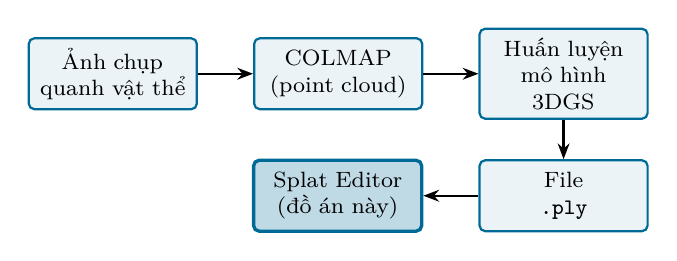
\begin{tikzpicture}[
  node distance=5mm and 7mm,
  box/.style={draw=linkblue,thick,rounded corners=2pt,fill=linkblue!8,align=center,
              minimum height=9mm,text width=19mm,font=\footnotesize},
  mine/.style={box,fill=linkblue!25,very thick},
  arr/.style={-{Stealth[length=2mm]},thick}]
  \node[box] (photos) {Ảnh chụp\\quanh vật thể};
  \node[box,right=of photos] (colmap) {COLMAP\\(point cloud)};
  \node[box,right=of colmap] (train) {Huấn luyện\\mô hình 3DGS};
  \node[box,below=of train] (ply) {File\\\code{.ply}};
  \node[mine,left=of ply] (editor) {Splat Editor\\(đồ án này)};
  \draw[arr] (photos) -- (colmap);
  \draw[arr] (colmap) -- (train);
  \draw[arr] (train) -- (ply);
  \draw[arr] (ply) -- (editor);
\end{tikzpicture}
\caption{Quy trình từ ảnh chụp đến Splat Editor. COLMAP \cite{schonberger2016colmap} tìm vị trí các camera.}
\label{fig:pipeline}
\end{figure}

Đồ án có hai phần. Phần một là pipeline hiển thị 3DGS, từ file đến shader. Phần hai là sáu nhóm kỹ thuật của môn học (Bảng~\ref{tab:map}).

\begin{table}[H]
\centering
\caption{Các nhóm kỹ thuật và các mục.}
\label{tab:map}
\footnotesize
\begin{tabular}{@{}lll@{}}
\toprule
Nhóm & Nội dung chính & Mục \\
\midrule
T1 & layer, ma trận $\mathbf{M}$, bộ xương nhân vật & \ref{chap:t1} \\
T2 & ma trận nhìn/chiếu, EWA, trộn alpha, camera & \ref{chap:t2} \\
T3 & texture skin của nhân vật & \ref{chap:t3} \\
T4 & màu SH, Phong, shadow map & \ref{chap:t4} \\
T5 & ngày--đêm, va chạm, hoạt họa nhân vật & \ref{chap:t5} \\
T6 & cọ chọn, xóa/hoàn tác, ImGui, HUD & \ref{chap:t6} \\
\bottomrule
\end{tabular}
\end{table}

\subsection{Cấu trúc chương trình}
Mã nguồn chia theo vai trò: \code{core} chỉ chứa dữ liệu và toán nên không phụ thuộc OpenGL, \code{render} chứa mọi lệnh OpenGL và shader, \code{ui} lo giao diện, còn \code{app.py} nối các phần lại. Hình~\ref{fig:tree} chỉ liệt kê các file đại diện.

\begin{figure}[H]
\centering
\begin{Verbatim}[fontsize=\fontsize{5.6}{6.6}\selectfont,frame=single]
SplatOpenGL/
|-- main.py              # điểm vào: python main.py [scene.ply]
|-- requirements.txt     # numpy, PyOpenGL, glfw, imgui-bundle
|-- report/              # báo cáo LaTeX
`-- splat_editor/
    |-- app.py           # vòng lặp chính, nối các phần lại
    |-- core/            # dữ liệu và toán, không dùng OpenGL
    |   |-- splats.py    # các mảng gaussian
    |   |-- layer.py     # một file PLY + biến đổi + vùng chọn
    |   |-- scene.py     # tập các layer
    |   |-- math3d.py    # ma trận V, P, góc Euler, quaternion
    |   |-- lighting.py  # mặt trời, đèn, ngày đêm
    |   |-- physics.py   # va chạm voxel, nhảy
    |   |-- avatar_pose.py  # góc khớp nhân vật
    |   |-- lod.py       # chọn gaussian theo mức chi tiết
    |   `-- history.py   # hoàn tác (undo)
    |-- io/              # đọc / ghi file
    |   |-- ply.py       # đọc / ghi PLY
    |   `-- codec.py     # cột PLY <-> Splats
    |-- editor/          # chỉnh sửa
    |   |-- editor.py    # mở, lưu, xoá, chọn
    |   `-- brush.py     # cọ chọn gaussian
    |-- render/          # OpenGL
    |   |-- splat_renderer.py  # vẽ gaussian (2 pass)
    |   |-- sorter.py    # sắp xếp độ sâu (luồng nền)
    |   |-- camera.py    # camera quỹ đạo / bay
    |   |-- avatar_renderer.py # vẽ nhân vật
    |   |-- shader.py    # biên dịch GLSL
    |   |-- shaders/     # splat_prep.vert, splat.vert/.frag, ...
    |   `-- textures/    # skinzom.png
    `-- ui/              # giao diện ImGui
        |-- window.py    # cửa sổ GLFW
        |-- input.py     # bàn phím, chuột
        `-- sections.py  # các bảng điều khiển
\end{Verbatim}
\caption{Cây thư mục của chương trình (chỉ các file chính).}
\label{fig:tree}
\end{figure}

\subsection{Dữ liệu đầu vào}
\label{sec:input}
Đầu vào là một file \code{.ply} do quá trình huấn luyện 3DGS tạo ra. Huấn luyện bắt đầu từ point cloud của COLMAP và đặt một gaussian tại mỗi điểm. Sau đó nó lặp lại ba bước. Nó vẽ các gaussian. Nó so ảnh vẽ ra với ảnh chụp thật. Nó cập nhật tham số của từng gaussian. Nó cũng xóa các gaussian vô ích và tách các gaussian quá lớn.

File có hai phần: header dạng văn bản và phần thân nhị phân. Header liệt kê các thuộc tính. Phần thân có một bản ghi cho mỗi gaussian. Mỗi giá trị là một số thực 32 bit. Bảng~\ref{tab:ply} liệt kê các thuộc tính. Với SH bậc 3, một bản ghi có 62 giá trị, tức 248 byte. Hình~\ref{fig:csv} là các dòng đầu của một file, xuất ra CSV.

\begin{table}[H]
\centering
\caption{Các thuộc tính của một gaussian trong file PLY.}
\label{tab:ply}
\footnotesize
\begin{tabular}{@{}p{2.3cm}p{0.9cm}p{4.4cm}@{}}
\toprule
Thuộc tính & Số & Ý nghĩa \\
\midrule
\code{x, y, z} & 3 & tâm $\symbf{\mu}$ \\
\code{nx, ny, nz} & 3 & pháp tuyến, luôn bằng 0, không dùng \\
\code{f\_dc\_0..2} & 3 & màu cơ bản (SH bậc 0) \\
\code{f\_rest\_*} & 45 & hệ số SH bậc 1--3 \\
\code{opacity} & 1 & độ đục thô \\
\code{scale\_0..2} & 3 & logarit của kích thước \\
\code{rot\_0..3} & 4 & quaternion quay \\
\bottomrule
\end{tabular}
\end{table}

\begin{figure}[H]
\centering
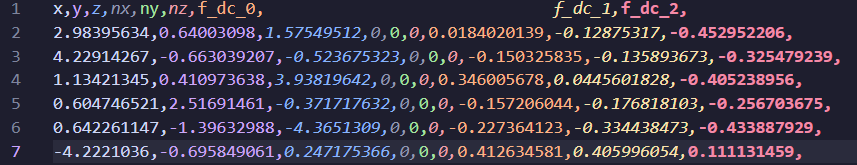
\includegraphics[width=\columnwidth]{figures/csv_head.png}\\[2pt]
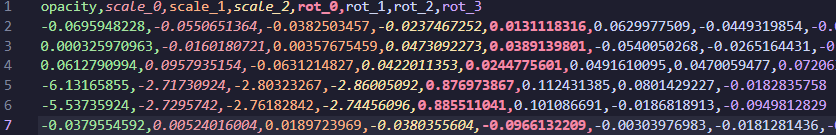
\includegraphics[width=\columnwidth]{figures/csv_tail.png}
\caption{Sáu gaussian đầu tiên của một file PLY, hiển thị dạng CSV. Trên: vị trí, pháp tuyến và màu cơ bản. Dưới: độ đục, kích thước và phép quay. Các cột \code{f\_rest} ở giữa được ẩn đi.}
\label{fig:csv}
\end{figure}

Chương trình ánh xạ file nhị phân thẳng vào bộ nhớ. Vì vậy file có hàng triệu gaussian mở gần như tức thì. Hình~\ref{fig:viewer} là một bản chụp nhỏ của một người. Các đốm mờ quanh người là gaussian lơ lửng mà trình chỉnh sửa phải xóa. Cảnh thử nghiệm chính là một con phố có khoảng 5 triệu gaussian (Hình~\ref{fig:scene}).

\begin{figure}[H]
\centering
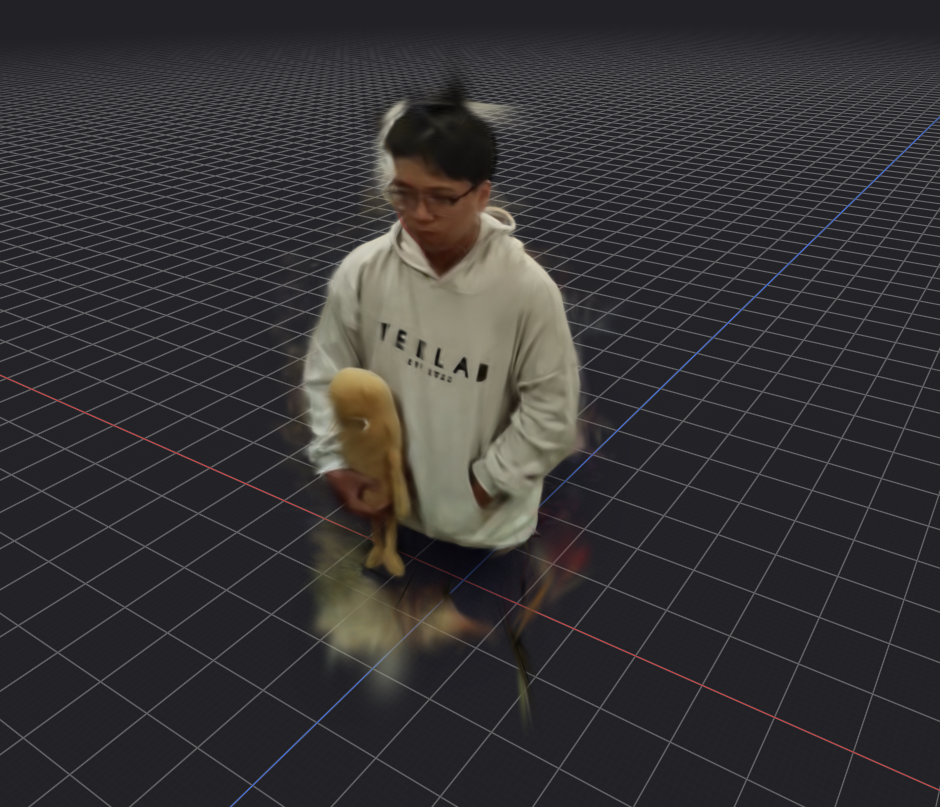
\includegraphics[width=0.6\columnwidth]{figures/viewer.png}
\caption{File PLY của một người được chụp lại. Các gaussian lơ lửng hiện rõ quanh người và gần mặt đất.}
\label{fig:viewer}
\end{figure}

\begin{figure}[H]
\centering
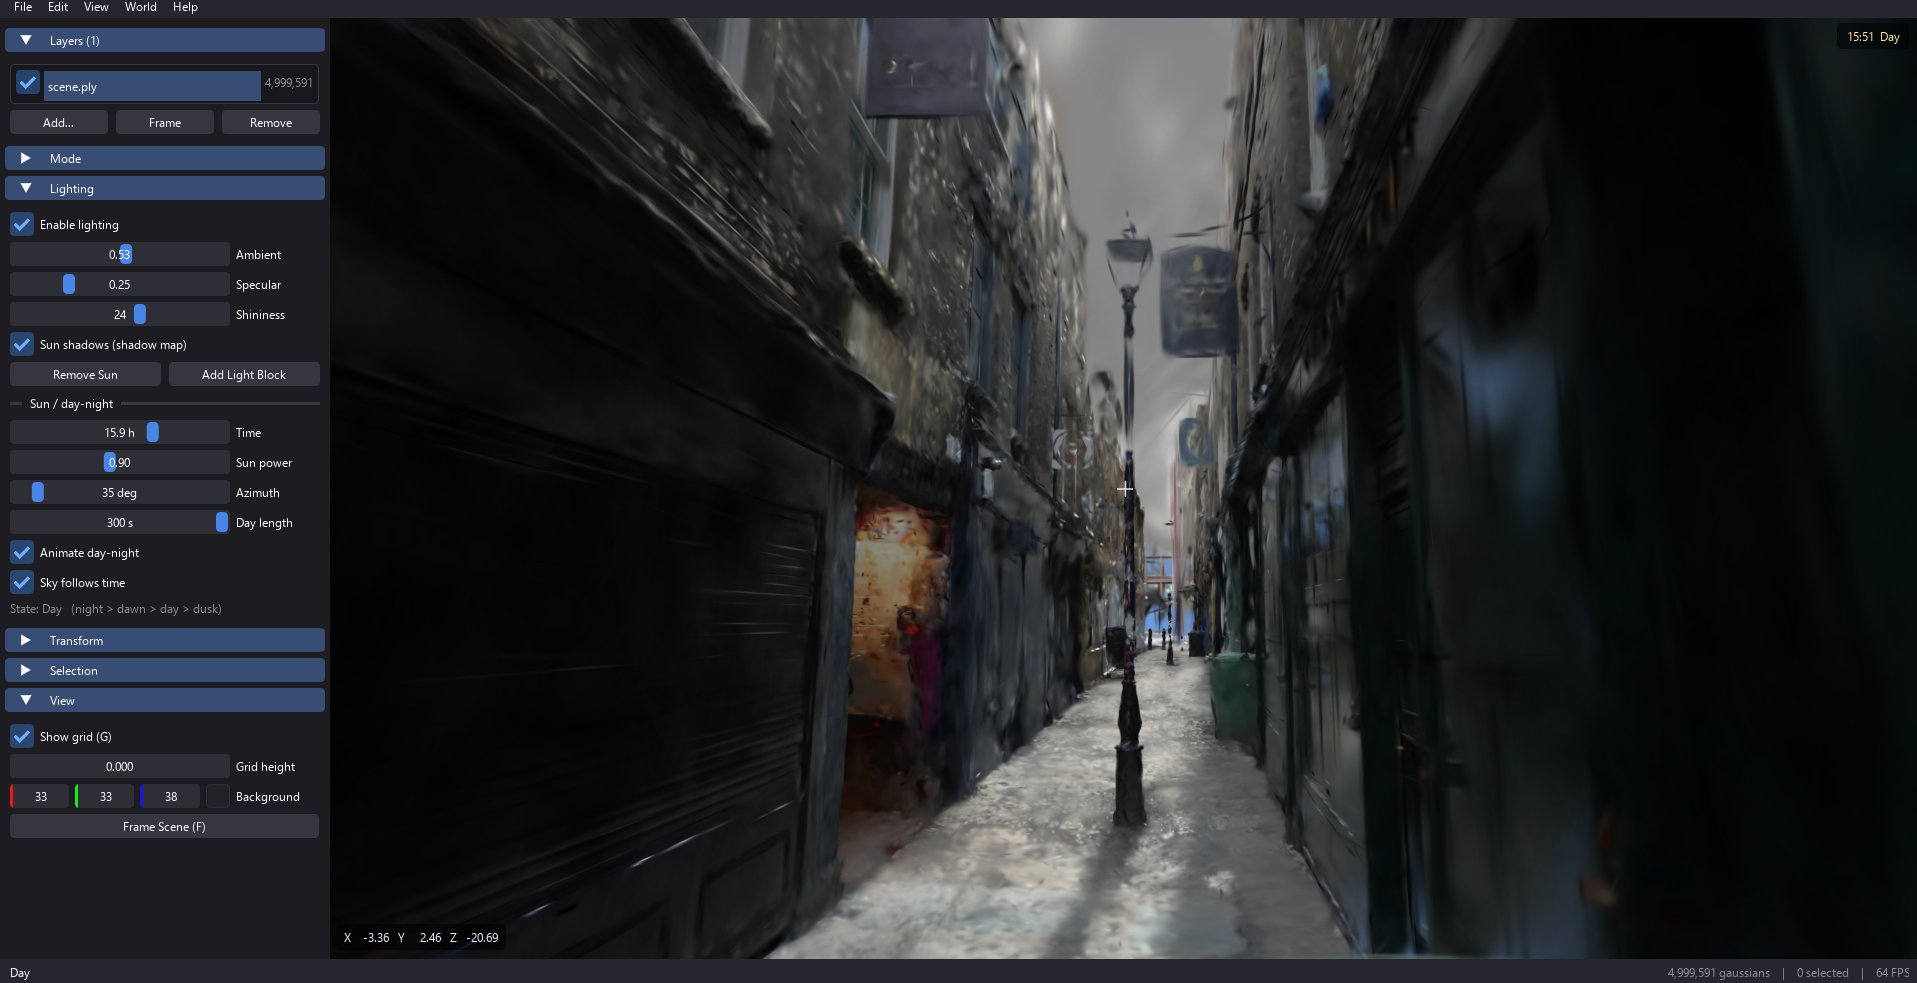
\includegraphics[width=\columnwidth]{figures/t4-day.png}\\[3pt]
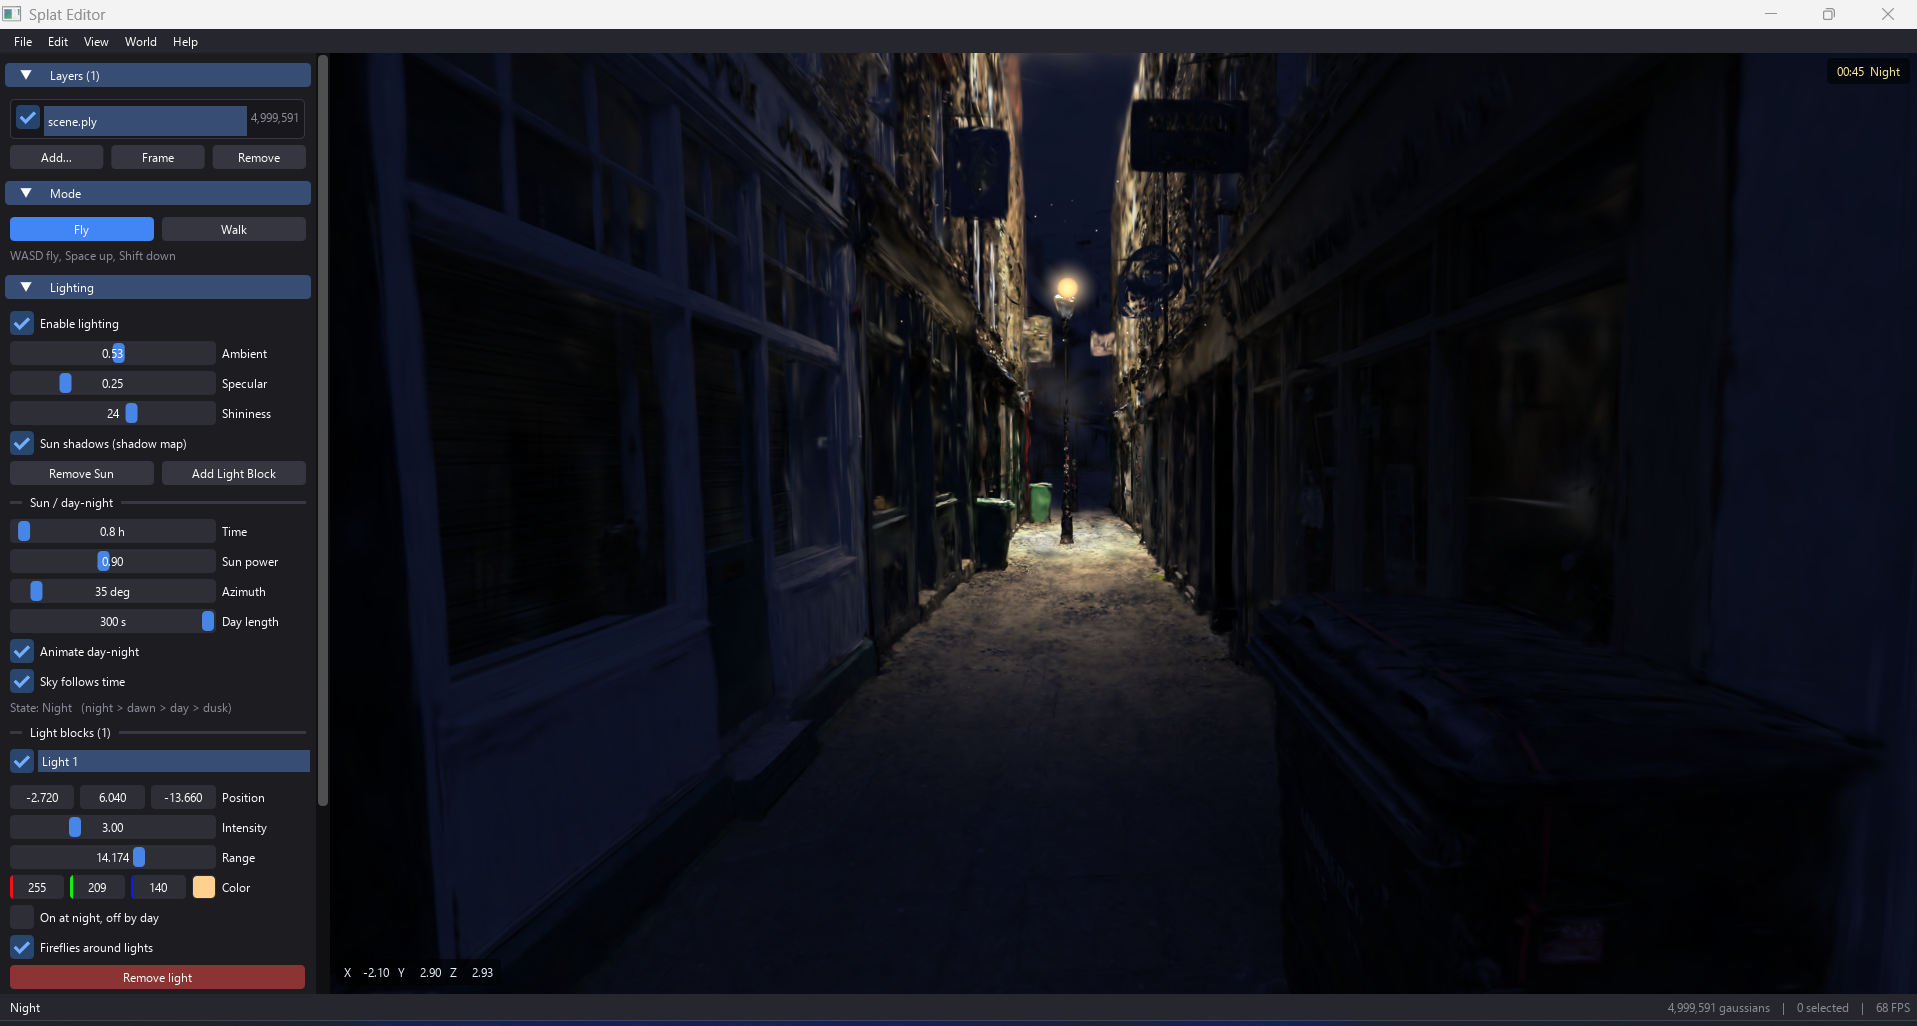
\includegraphics[width=\columnwidth]{figures/t4-night.png}
\caption{Một cảnh khoảng 5 triệu gaussian trong Splat Editor, ban ngày (trên) và ban đêm (dưới).}
\label{fig:scene}
\end{figure}

\subsection{Gaussian và file PLY}
\label{sec:decode}
Mỗi gaussian có vị trí $\symbf{\mu}$, màu $\mathbf{c}$, độ đục $\alpha$, kích thước $\mathbf{s}$ và phép quay $\symbf{q}$ (quaternion). Mật độ của nó giảm dần từ tâm ra ngoài. Ta có thể hình dung nó là một ellipsoid (Hình~\ref{fig:g2e}). File PLY lưu giá trị thô. Chương trình giải mã khi đọc:
\begin{itemize}\itemsep0pt
  \item Kích thước: $s_i=\exp(\code{scale\_i})$.
  \item Độ đục: $\alpha=1/(1+e^{-\code{opacity}})$.
  \item Màu: $\mathrm{RGB}=0{,}5+C_0\,\code{f\_dc}$, với $C_0\approx0{,}2821$.
  \item Phép quay: chuẩn hóa quaternion \code{rot\_0..3} về độ dài 1.
\end{itemize}
Khi lưu file, chương trình làm ngược lại.

\begin{codebox}
\begin{lstlisting}[language=Python,caption={\code{io/codec.py}, \code{SplatCodec.decode}: giải mã giá trị thô của file PLY},label={lst:decode}]
SH_C0 = 0.28209479177387814
colors = 0.5 + SH_C0 * np.stack([col('f_dc_0'), col('f_dc_1'), col('f_dc_2')], axis=1)
alphas = 1.0 / (1.0 + np.exp(-col('opacity')))
scales = np.exp(np.stack([col('scale_0'), col('scale_1'), col('scale_2')], axis=1))
q = np.stack([col('rot_0'), col('rot_1'), col('rot_2'), col('rot_3')], axis=1)
length = np.linalg.norm(q, axis=1, keepdims=True)
q = q / np.maximum(length, 1e-12)
\end{lstlisting}
\end{codebox}

\begin{figure}[H]
\centering
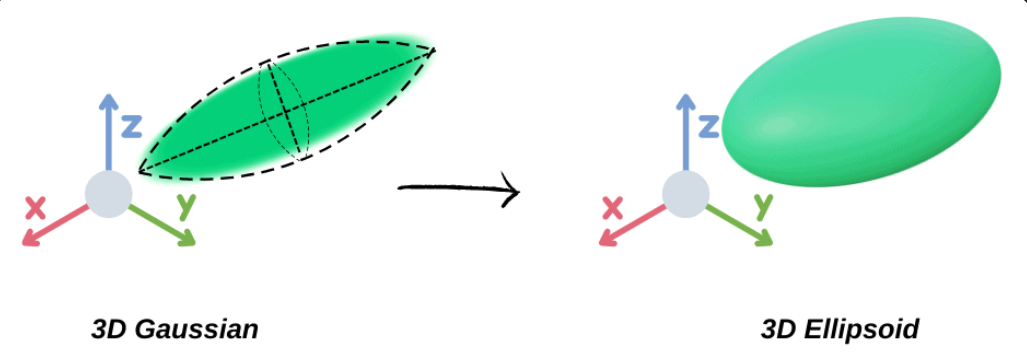
\includegraphics[width=\columnwidth]{figures/1 (4).png}
\caption{Gaussian 3D là một đốm mềm. Mặt của nó tại một độ lệch chuẩn là một ellipsoid.}
\label{fig:g2e}
\end{figure}

Hình dạng của gaussian nằm trong ma trận hiệp phương sai $\Sig$. Nó được tạo từ ma trận co giãn $\mathbf{S}=\mathrm{diag}(\mathbf{s})$ và ma trận quay $\mathbf{R}(\symbf{q})$:
\begin{equation}
\Sig=\mathbf{R}\,\mathbf{S}\mathbf{S}^{\top}\mathbf{R}^{\top}.
\label{eq:cov3d}
\end{equation}
Hình~\ref{fig:rs} cho hai ma trận này. Hình~\ref{fig:ellipsoid} vẽ kết quả cho gaussian đầu tiên của Hình~\ref{fig:csv}. Ba kích thước $s_0,s_1,s_2$ là các bán trục của ellipsoid. Quaternion xoay các trục này trong không gian. Mục~\ref{sec:ewa} chiếu ellipsoid này lên màn hình.

\begin{codebox}
\begin{lstlisting}[language=GLSL,caption={\code{render/shaders/splat\_prep.vert}: dựng $\Sigma=\mathbf{R}\mathbf{S}\mathbf{S}^{\top}\mathbf{R}^{\top}$},label={lst:cov3d}]
vec3 scale = vec3(unpackHalf(t1.y), halfToFloat(t1.z & 65535u));
vec4 q = normalize((vec4(uvec4(t1.w, t1.w >> 8u, t1.w >> 16u, t1.w >> 24u)
                         & 255u) - 128.0) / 127.0);
float w = q.x, x = q.y, y = q.z, z = q.w;
mat3 R = mat3(1.0 - 2.0 * (y * y + z * z), 2.0 * (x * y + w * z), 2.0 * (x * z - w * y),
              2.0 * (x * y - w * z), 1.0 - 2.0 * (x * x + z * z), 2.0 * (y * z + w * x),
              2.0 * (x * z + w * y), 2.0 * (y * z - w * x), 1.0 - 2.0 * (x * x + y * y));
mat3 M = R * mat3(scale.x, 0.0, 0.0, 0.0, scale.y, 0.0, 0.0, 0.0, scale.z);
mat3 sigma = M * transpose(M);
\end{lstlisting}
\end{codebox}

\begin{figure}[H]
\centering
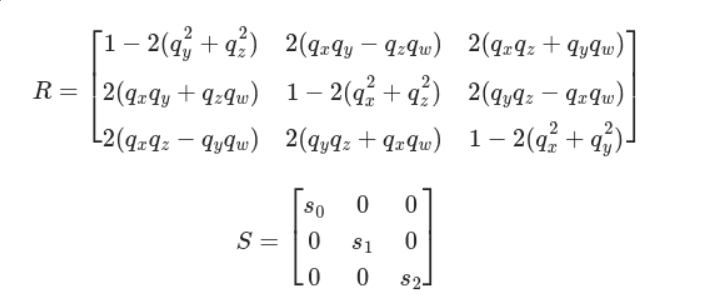
\includegraphics[width=0.75\columnwidth]{figures/1 (5).png}
\caption{Ma trận quay $\mathbf{R}$ từ quaternion $(q_w,q_x,q_y,q_z)$ và ma trận co giãn $\mathbf{S}$.}
\label{fig:rs}
\end{figure}

\begin{figure}[H]
\centering
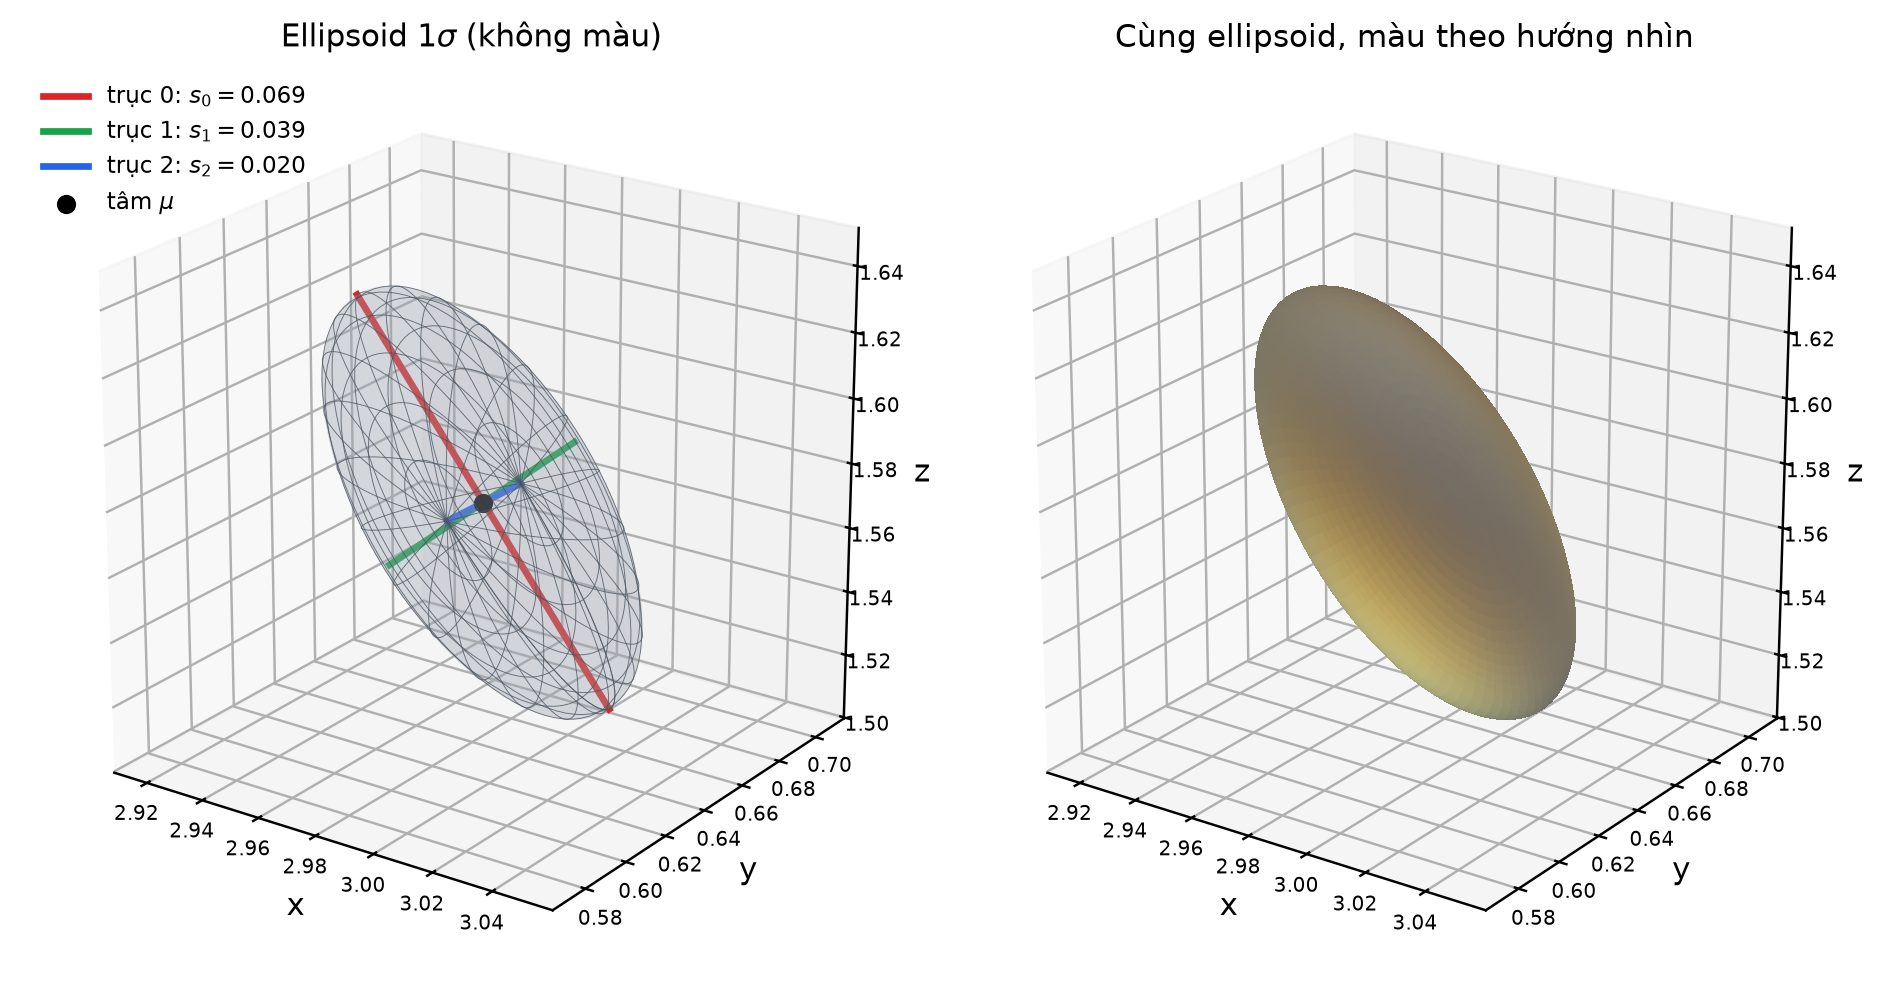
\includegraphics[width=\columnwidth]{figures/example_ellipsoid.png}
\caption{Một gaussian trong file. Trái: ellipsoid $1\sigma$ với ba trục và tâm $\symbf{\mu}$. Phải: cùng ellipsoid đó với màu phụ thuộc hướng nhìn.}
\label{fig:ellipsoid}
\end{figure}


\begin{figure*}[t]
\centering
\begin{minipage}{0.495\textwidth}\centering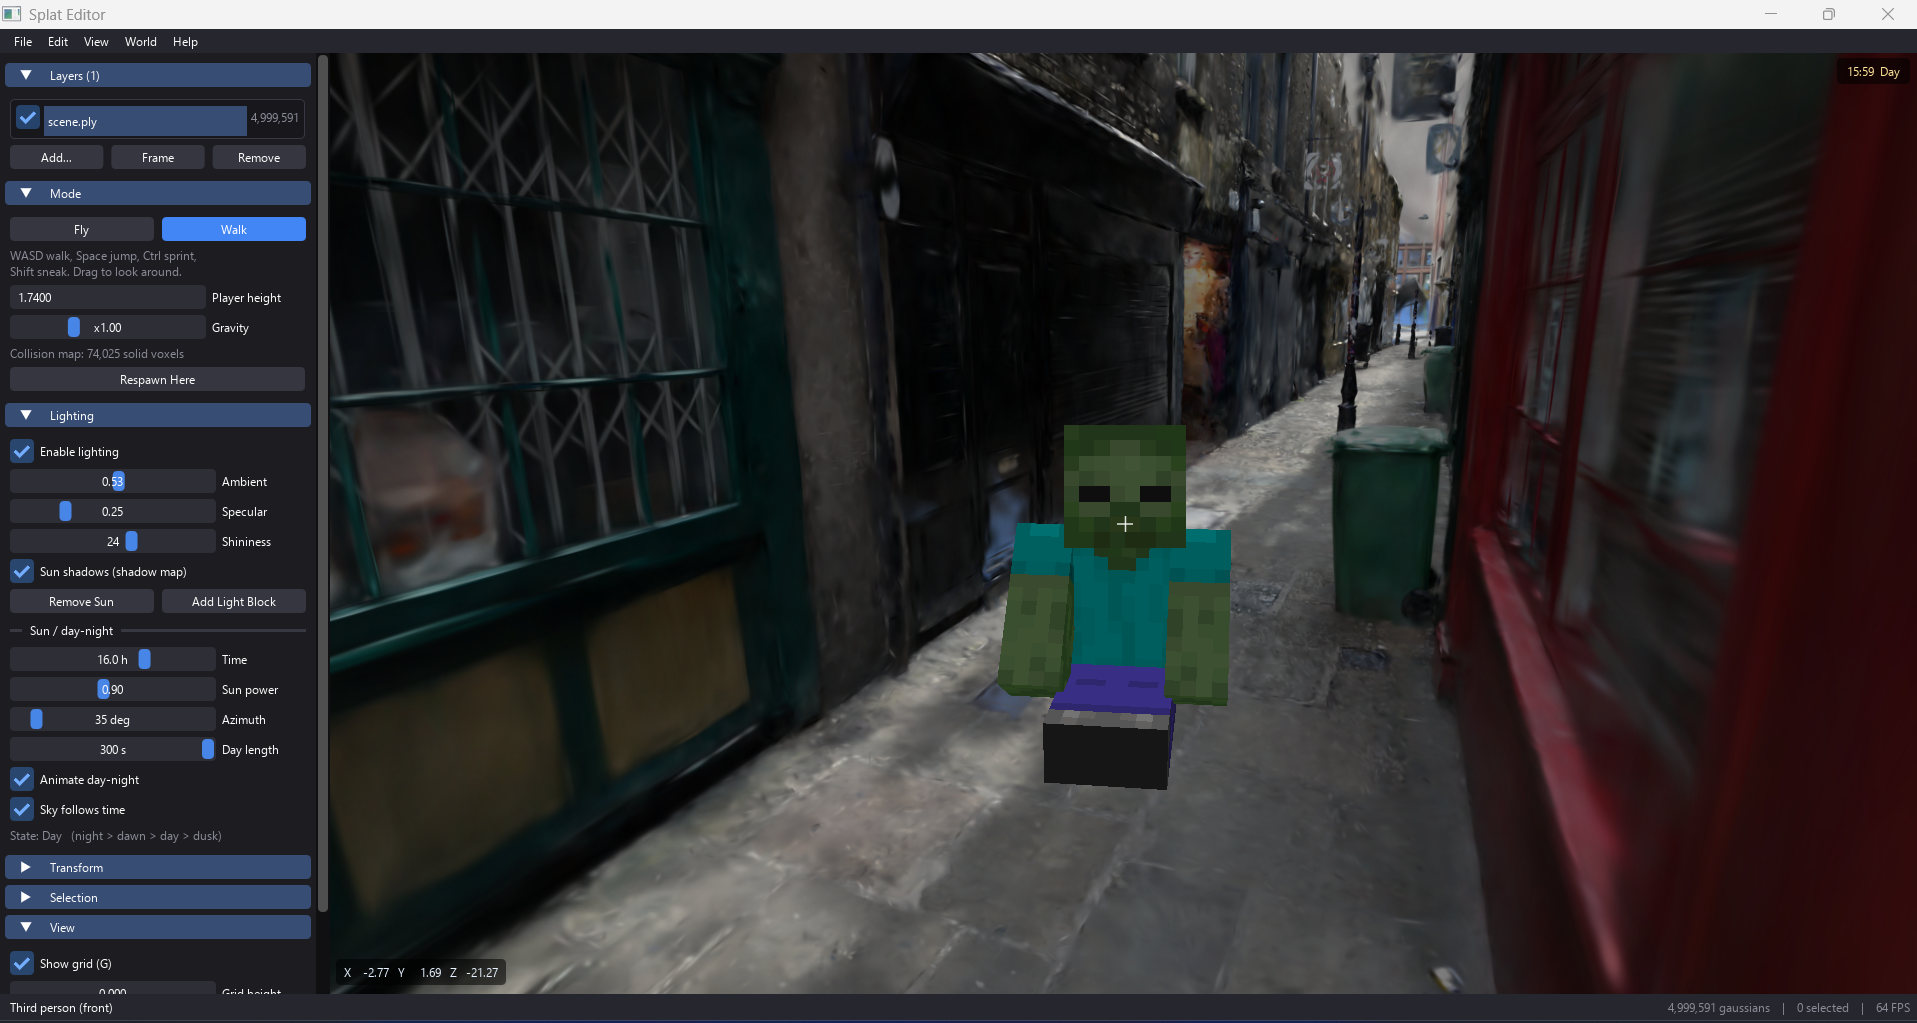
\includegraphics[width=\linewidth]{figures/t4-zombie-day.png}\\{\footnotesize (a) Ban ngày, 15:59.}\end{minipage}\hfill
\begin{minipage}{0.495\textwidth}\centering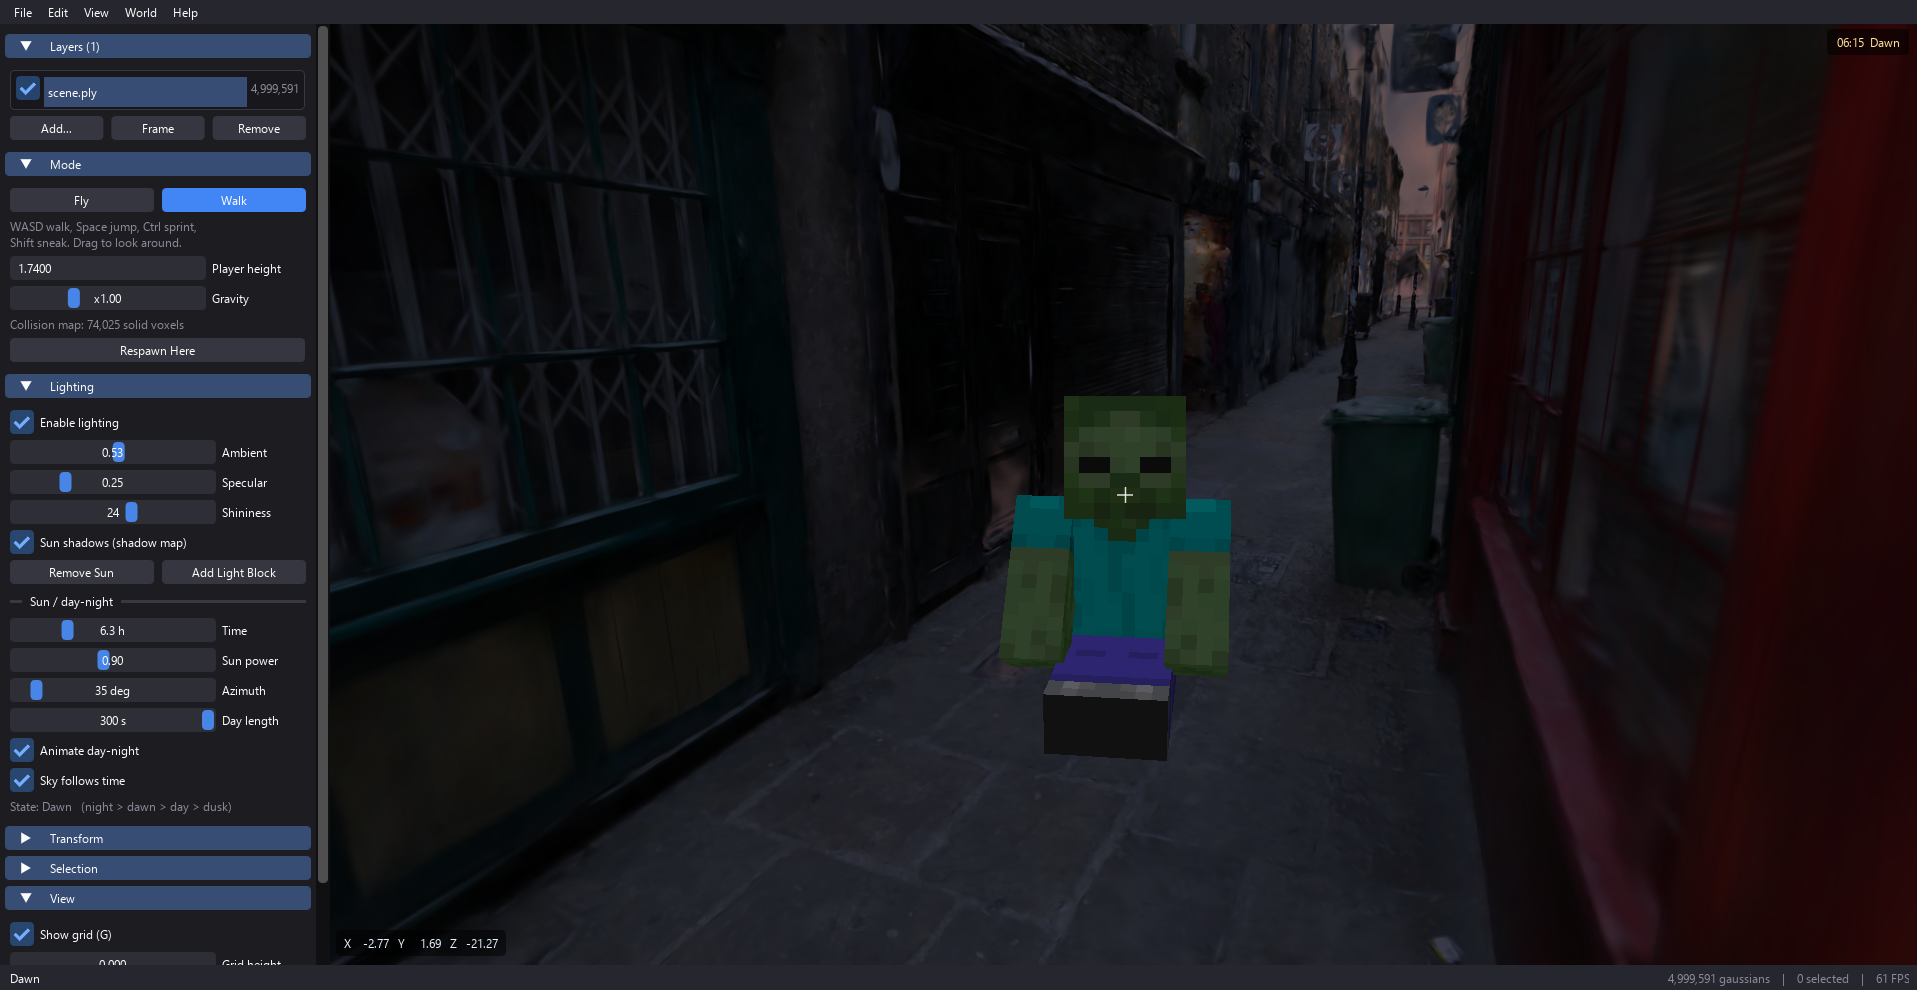
\includegraphics[width=\linewidth]{figures/t4-dawn.png}\\{\footnotesize (b) Bình minh, 06:15.}\end{minipage}\\[5pt]
\begin{minipage}{0.495\textwidth}\centering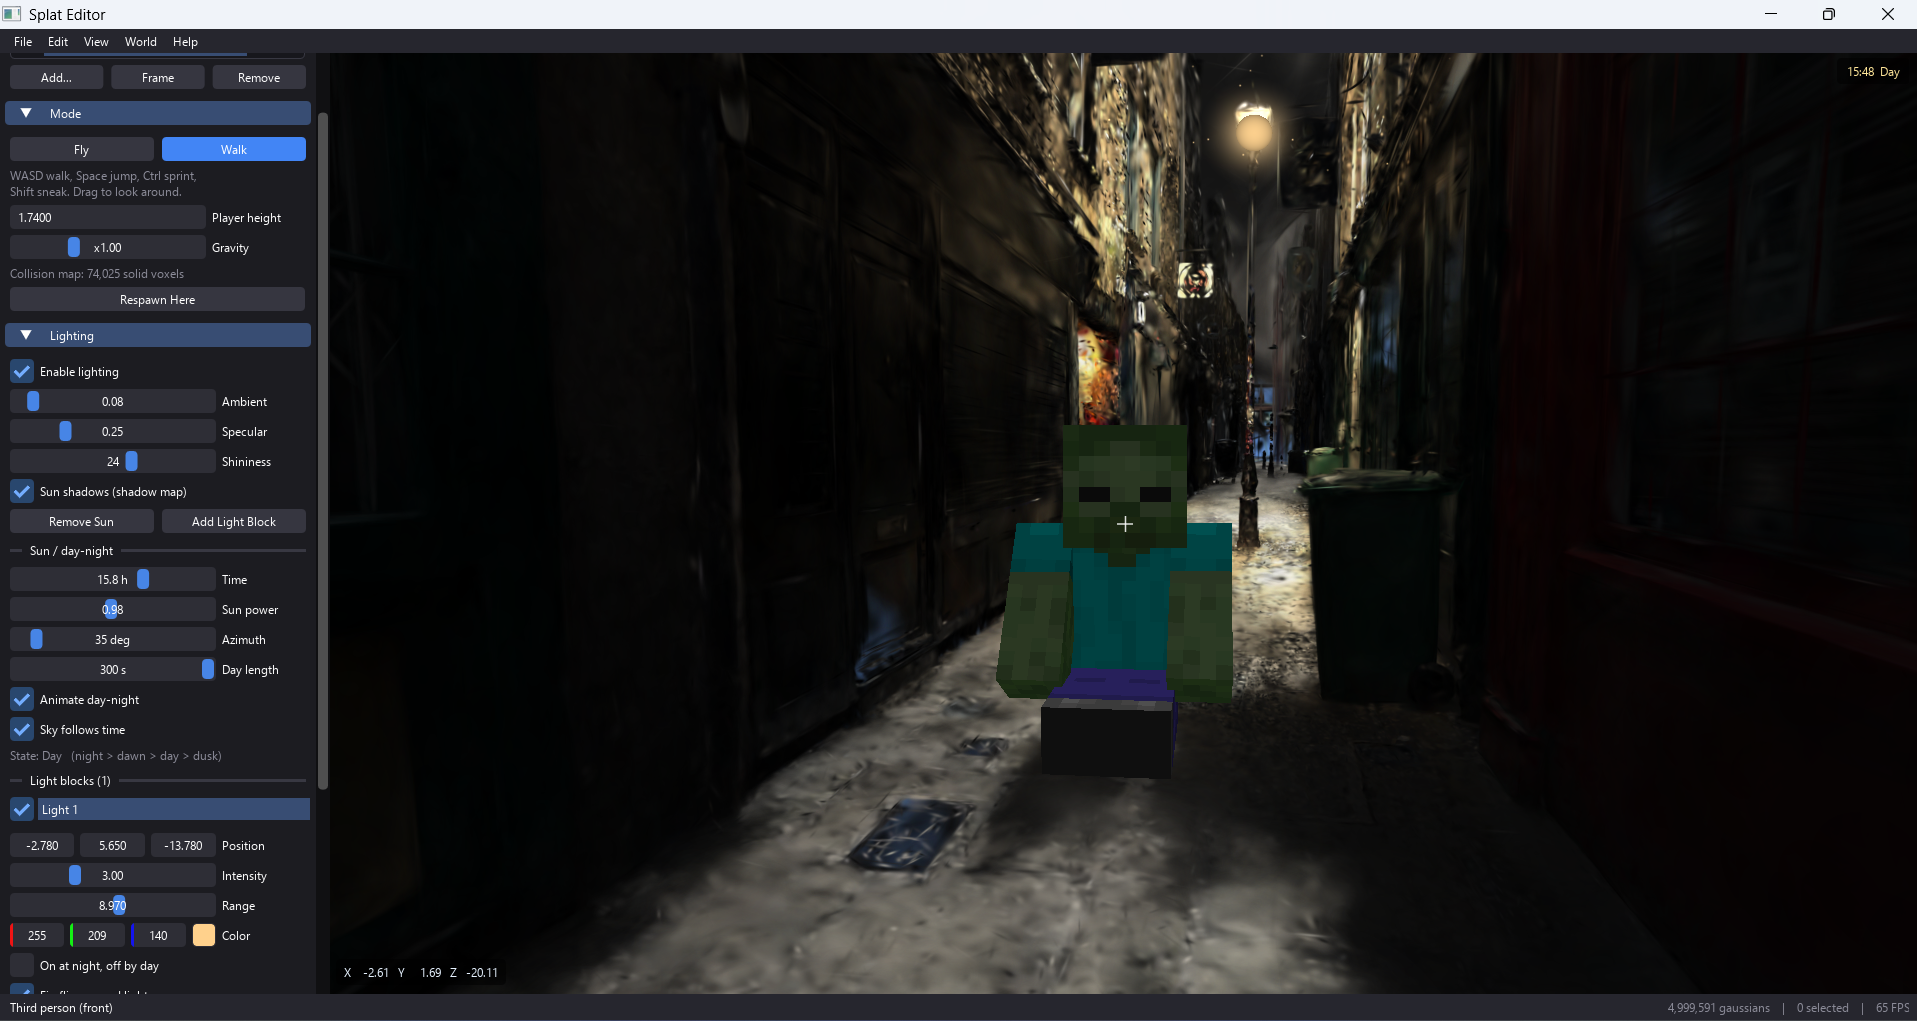
\includegraphics[width=\linewidth]{figures/t4-lamp-zombie.png}\\{\footnotesize (c) Môi trường $0{,}08$ và một đèn.}\end{minipage}\hfill
\begin{minipage}{0.495\textwidth}\centering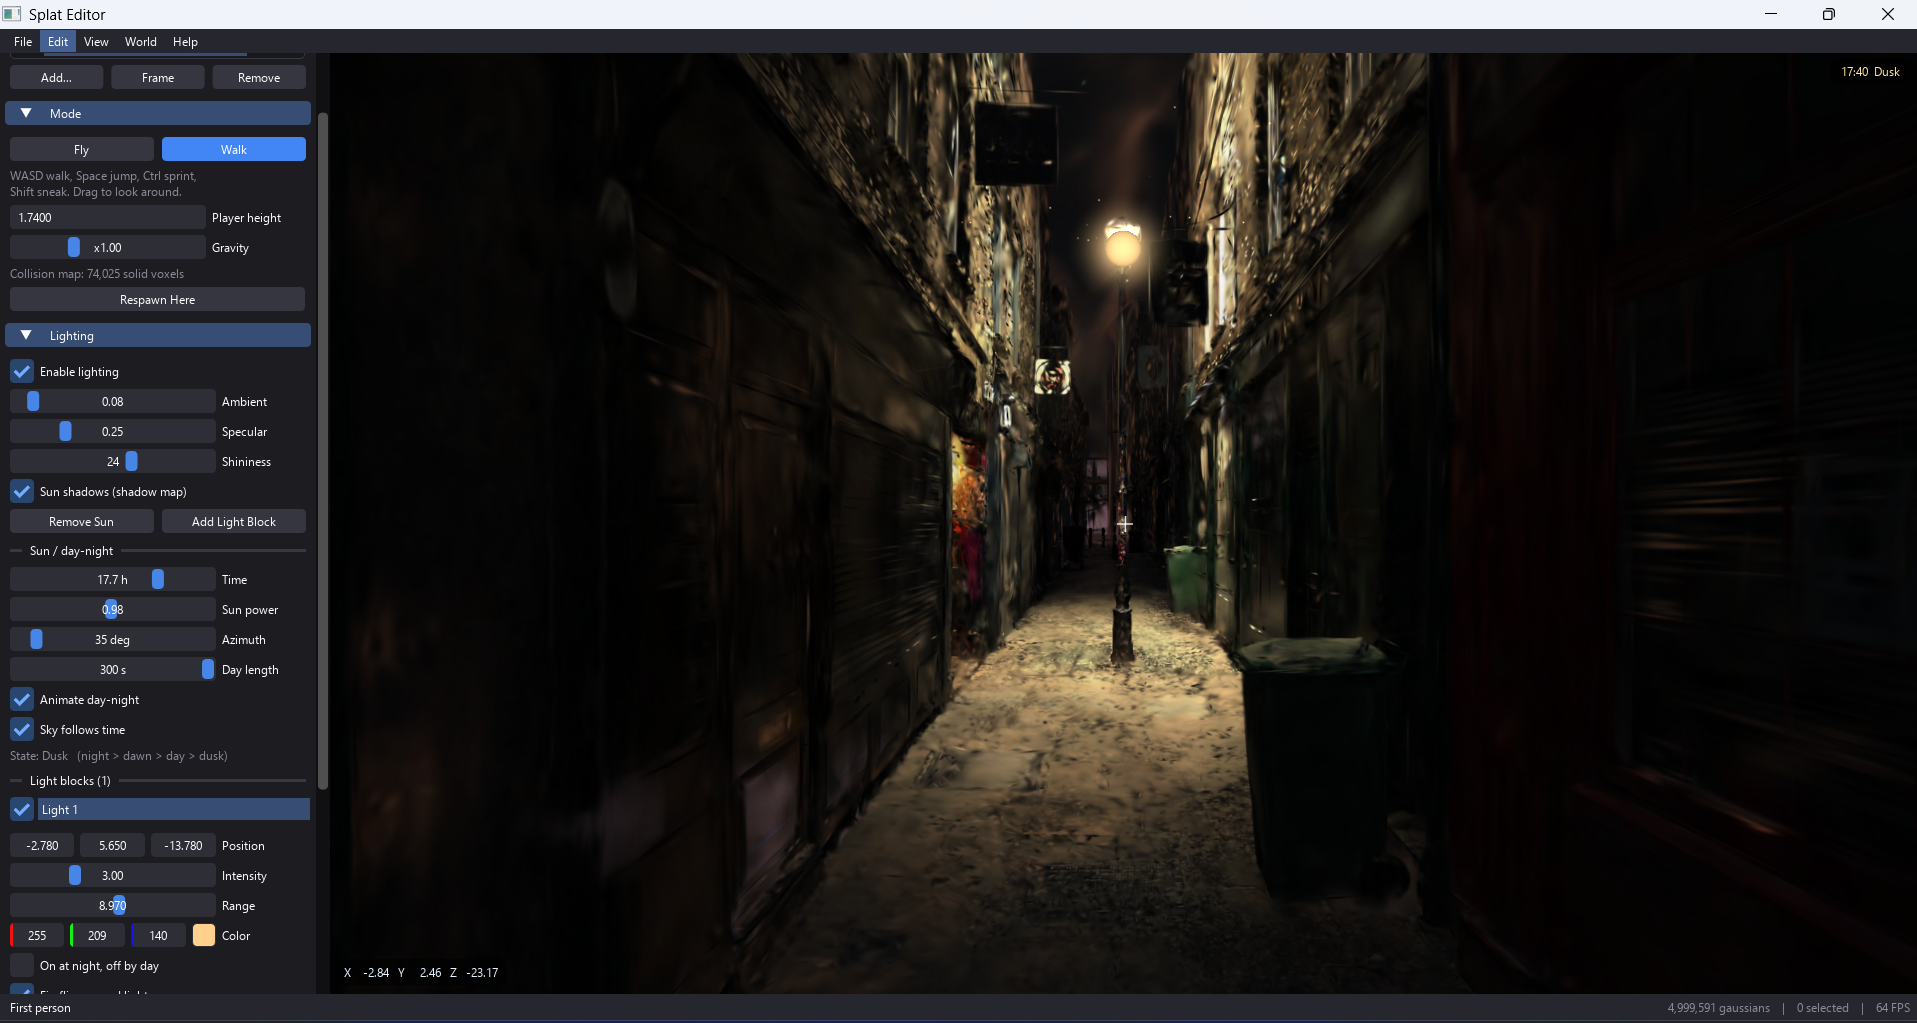
\includegraphics[width=\linewidth]{figures/t4-dusk.png}\\{\footnotesize (d) Hoàng hôn, 17:40.}\end{minipage}
\caption{Cảnh có mặt trời, một đèn điểm và nhân vật vào các giờ khác nhau trong ngày.}
\label{fig:t4}
\end{figure*}


%====================================================================
\section{T1: Phép biến đổi và mô hình phân cấp}
\label{chap:t1}
%====================================================================
Chương này có ba phần. Hai phần đầu di chuyển cả một layer, phần cuối di chuyển một mô hình phân cấp.
\begin{itemize}\itemsep0pt
\item \textbf{Phần 1, biến đổi layer.} Đưa gaussian của một file \code{.ply} vào thế giới.
\item \textbf{Phần 2, quay quanh một điểm.} Quay layer quanh một tâm tùy chọn.
\item \textbf{Phần 3, bộ xương nhân vật.} Dựng ma trận của nhân vật từ một cây khớp.
\end{itemize}

\subsection{Phần 1: Biến đổi layer}
\label{sec:layers}
Mỗi file \code{.ply} là một layer. Layer có vector tịnh tiến $\mathbf{t}$, ba góc Euler và hệ số co giãn $s$. Chúng tạo thành ma trận $\mathbf{M}$. Ma trận này đưa gaussian từ không gian file sang thế giới:
\begin{equation}
\mathbf{p}_w=s\mathbf{A}\mathbf{p}_f+\mathbf{t},\qquad
\Sig_w=s^{2}\mathbf{A}\,\Sig_f\,\mathbf{A}^{\top}.
\label{eq:world}
\end{equation}
Ở đây $\mathbf{A}=\mathbf{R}_z\mathbf{R}_y\mathbf{R}_x\mathbf{F}$. $\mathbf{F}=\mathrm{diag}(-1,-1,1)$ là phép lật tùy chọn cho file COLMAP có trục $Y$ hướng xuống. Dữ liệu gaussian không đổi. Chỉ $\mathbf{M}$ thay đổi. Vì vậy di chuyển, xoay hoặc co giãn một layer diễn ra tức thì. Khi lưu, chương trình ghi phép biến đổi vào từng gaussian. Nó cũng xoay các hệ số SH để màu theo hướng nhìn vẫn đúng.

\begin{codebox}
\begin{lstlisting}[language=Python,caption={\code{core/math3d.py} và \code{core/layer.py}: ma trận $\mathbf{M}$ của layer},label={lst:world}]
rx = np.array([[1, 0, 0], [0, cx, -sx], [0, sx, cx]])
ry = np.array([[cy, 0, sy], [0, 1, 0], [-sy, 0, cy]])
rz = np.array([[cz, -sz, 0], [sz, cz, 0], [0, 0, 1]])
return rz @ ry @ rx

rot = self.transform.rotation_matrix() @ (FLIP if flip else np.identity(3))
m = np.identity(4)
m[:3, :3] = s * rot
m[:3, 3] = t
\end{lstlisting}
\end{codebox}

\subsection{Phần 2: Quay quanh một điểm}
Layer có thể quay quanh điểm $\mathbf{c}$ bằng ma trận $\symbf{\Delta}$:
\begin{equation}
\mathbf{R}'=\symbf{\Delta}\mathbf{R},\qquad \mathbf{t}'=\symbf{\Delta}(\mathbf{t}-\mathbf{c})+\mathbf{c}.
\end{equation}

\begin{codebox}
\begin{lstlisting}[language=Python,caption={\code{core/transform.py}, \code{Transform.rotate\_about}},label={lst:pivot}]
def rotate_about(self, delta, pivot):
    pivot = np.asarray(pivot, float)
    self.rotation = matrix_to_euler(delta @ self.rotation_matrix())
    self.position = list(delta @ (self.translation() - pivot) + pivot)
\end{lstlisting}
\end{codebox}

\subsection{Phần 3: Bộ xương nhân vật}
\label{sec:skeleton}
Nhân vật hiện ra khi bấm \code{F5}. Nó có sáu hộp: đầu, thân, hai tay và hai chân. Mỗi hộp có một ma trận riêng. Ma trận này là tích các ma trận khớp từ gốc xuống (Hình~\ref{fig:skeleton}). Mỗi khớp quay quanh một điểm $\mathbf{p}$:
\begin{equation}
\mathbf{M}_{\text{con}}=\mathbf{M}_{\text{cha}}\,\mathbf{T}(\mathbf{p})\,\mathbf{R}\,\mathbf{T}(-\mathbf{p}).
\end{equation}
Chân là con của gốc. Tay và đầu là con của thân, nên chúng nghiêng theo thân. Các góc khớp đến từ hoạt họa (Mục~\ref{chap:t5}).

\begin{codebox}
\begin{lstlisting}[language=Python,caption={\code{core/avatar\_pose.py}, \code{limb\_matrices}: ma trận khớp},label={lst:joint}]
def leg(angle):
    return (root @ _translate(0, HIP_Y, 0) @ _rot("x", angle)
            @ _translate(0, -HIP_Y, 0))

def arm(px, angles):
    return (upper @ _translate(px, SHOULDER_Y, 0) @ _rot("z", angles[1])
            @ _rot("x", angles[0]) @ _translate(-px, -SHOULDER_Y, 0))
\end{lstlisting}
\end{codebox}

\begin{figure}[H]
\centering
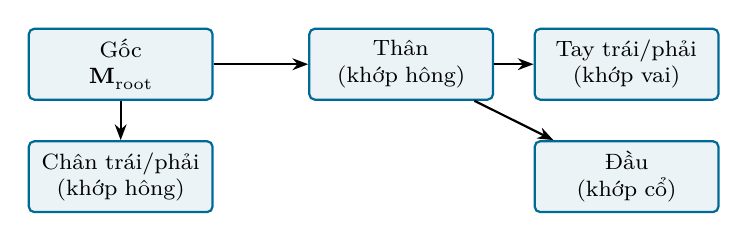
\begin{tikzpicture}[node distance=5mm and 5mm]
  \node[pbox] (root) {Gốc\\$\mathbf{M}_{\text{root}}$};
  \node[pbox,right=12mm of root] (body) {Thân\\(khớp hông)};
  \node[pbox,below=of root] (leg) {Chân trái/phải\\(khớp hông)};
  \node[pbox,right=of body] (arm) {Tay trái/phải\\(khớp vai)};
  \node[pbox,below=of arm] (head) {Đầu\\(khớp cổ)};
  \draw[parr] (root) -- (body);
  \draw[parr] (root) -- (leg);
  \draw[parr] (body) -- (arm);
  \draw[parr] (body) -- (head);
\end{tikzpicture}
\caption{Cây phân cấp của nhân vật. Mỗi mũi tên là một phép nhân ma trận.}
\label{fig:skeleton}
\end{figure}


%====================================================================
\section{T2: Camera và phép chiếu}
\label{chap:t2}
%====================================================================
Một gaussian đi qua bốn bước để thành pixel trên màn hình \cite{zwicker2002ewa}. Mỗi bước là một ô trong Hình~\ref{fig:ewa}, đọc từ trái sang phải.
\begin{itemize}\itemsep0pt
\item \textbf{Phần 1, phép biến đổi nhìn} (\emph{viewing transformation}). Đưa gaussian từ không gian vật thể về không gian camera.
\item \textbf{Phần 2, phép chiếu} (\emph{projective mapping}). Biến ellipsoid 3D thành ellipse 2D.
\item \textbf{Phần 3, tô màu và trộn} (\emph{shading and integration}). Tính độ đục của từng pixel và trộn các gaussian với nhau.
\item \textbf{Phần 4, phép biến đổi vùng nhìn} (\emph{viewport transformation}). Đặt kết quả vào vùng nhìn của cửa sổ.
\end{itemize}
Năm phần dưới đây đi theo đúng thứ tự này.
\begin{figure}[H]
\centering
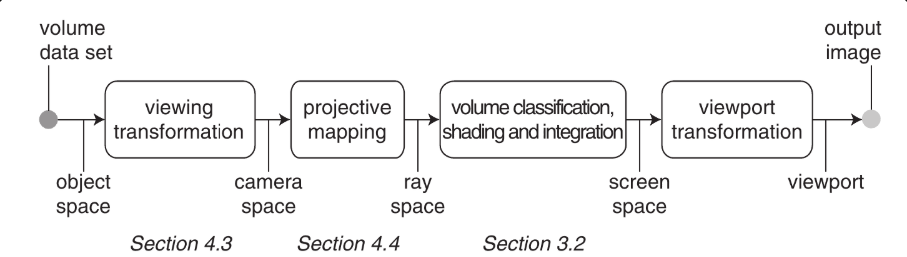
\includegraphics[width=\columnwidth]{figures/1 (3).png}
\caption{Pipeline splatting của EWA \cite{zwicker2002ewa}. Phép biến đổi nhìn là $\mathbf{W}$ và phép chiếu được xấp xỉ bằng $\mathbf{J}$.}
\label{fig:ewa}
\end{figure}

\subsection{Phần 1: Phép biến đổi nhìn}
\label{sec:cam}
Bước này đổi hệ tọa độ. Sau bước này, camera nằm ở gốc tọa độ và nhìn dọc theo trục $-z$. Hàm \code{look\_at} tạo ba trục camera từ vị trí mắt $\mathbf{e}$ và điểm nhìn: phải $\mathbf{r}$, lên $\mathbf{u}$ và trước $\mathbf{f}$. Ma trận nhìn là
\begin{equation}
\mathbf{V}=\begin{pmatrix}
\setlength{\fboxsep}{2pt}\fcolorbox{red}{white}{$\begin{matrix}
r_x&r_y&r_z\\u_x&u_y&u_z\\-f_x&-f_y&-f_z\end{matrix}$}
&\begin{matrix}-\mathbf{r}\!\cdot\!\mathbf{e}\\-\mathbf{u}\!\cdot\!\mathbf{e}\\ \mathbf{f}\!\cdot\!\mathbf{e}\end{matrix}\\[3mm]
\begin{matrix}0&0&0\end{matrix}&1\end{pmatrix}.
\label{eq:view}
\end{equation}
Tâm gaussian được nhân với $\mathbf{V}$. Kết quả là tâm trong không gian camera $(v_x,v_y,v_z)$. Hình dạng của gaussian chỉ bị quay. Ma trận $\mathbf{W}$ là phần quay của $\mathbf{V}$. Đó là khối $3\times3$ trên trái, trong ô vuông đỏ ở \eqref{eq:view}. Các hàng của nó là ba trục camera:
\begin{equation}
\mathbf{W}=\begin{pmatrix}
r_x&r_y&r_z\\u_x&u_y&u_z\\-f_x&-f_y&-f_z\end{pmatrix}.
\label{eq:W}
\end{equation}
Ellipsoid \eqref{eq:cov3d} trong không gian camera là $\mathbf{W}\,\Sig\,\mathbf{W}^{\top}$.

\begin{codebox}
\begin{lstlisting}[language=Python,caption={\code{core/math3d.py}, \code{look\_at}: ma trận nhìn $\mathbf{V}$},label={lst:lookat}]
def look_at(eye, target, up):
    forward = target - eye
    forward /= np.linalg.norm(forward)
    right = np.cross(forward, up)
    right /= np.linalg.norm(right)
    true_up = np.cross(right, forward)
    m = np.identity(4, np.float32)
    m[0, :3] = right
    m[1, :3] = true_up
    m[2, :3] = -forward
    m[:3, 3] = -m[:3, :3] @ eye
    return m
\end{lstlisting}
\end{codebox}

\subsection{Phần 2: Phép chiếu}
\label{sec:ewa}
Bước này đưa không gian camera lên mặt phẳng ảnh.

\textbf{Chiếu một điểm.} Ma trận chiếu phối cảnh dùng góc nhìn dọc $\varphi$ ($k=1/\tan(\varphi/2)$), tỉ lệ khung hình $a$, mặt phẳng gần $n$ và xa $f$:
\begin{equation}
\mathbf{P}=\begin{pmatrix}
\frac{k}{a}&0&0&0\\0&k&0&0\\
0&0&\frac{f+n}{n-f}&\frac{2fn}{n-f}\\0&0&-1&0\end{pmatrix}.
\label{eq:proj}
\end{equation}
Điểm được nhân với $\mathbf{P}$ rồi chia cho $c_w$. Kết quả là tọa độ chuẩn hóa $(n_x,n_y)$ trong khoảng $[-1,1]$. Phép chia cho $c_w$ làm vật ở xa trông nhỏ hơn. Tâm gaussian được chiếu theo cách này.

\begin{codebox}
\begin{lstlisting}[language=Python,caption={\code{core/math3d.py}, \code{perspective}: ma trận chiếu $\mathbf{P}$},label={lst:persp}]
def perspective(fov_y_deg, aspect, near, far):
    zoom = 1.0 / math.tan(math.radians(fov_y_deg) / 2)
    m = np.zeros((4, 4), np.float32)
    m[0, 0] = zoom / aspect
    m[1, 1] = zoom
    m[2, 2] = (far + near) / (near - far)
    m[2, 3] = 2 * far * near / (near - far)
    m[3, 2] = -1
    return m
\end{lstlisting}
\end{codebox}

\textbf{Chiếu một gaussian.} Gaussian không phải là một điểm. Ellipsoid của nó phải thành một ellipse trên màn hình. Phép chia cho $c_w$ không tuyến tính, nên không thể nhân $\mathbf{P}$ với ellipsoid. EWA thay phép chiếu bằng đạo hàm của nó (Jacobian) tại tâm gaussian:
\begin{equation}
\mathbf{J}=\begin{pmatrix}
\frac{f_{px}}{-v_z}&0&\frac{f_{px}\,v_x}{v_z^{2}}\\[1mm]
0&\frac{f_{px}}{-v_z}&\frac{f_{px}\,v_y}{v_z^{2}}\\[1mm]
0&0&0
\end{pmatrix}.
\label{eq:jac}
\end{equation}
Ở đây $f_{px}=kH/2$ là tiêu cự tính bằng pixel, với $k$ lấy từ \eqref{eq:proj} và $H$ là chiều cao vùng nhìn. Ghép bước 1 và bước 2, hiệp phương sai 2D là
\begin{equation}
\Sig'=\mathbf{J}\,\mathbf{W}\,\Sig\,\mathbf{W}^{\top}\mathbf{J}^{\top}.
\label{eq:ewa}
\end{equation}
Ở đây $\Sig$ là hiệp phương sai 3D \eqref{eq:cov3d}. $\mathbf{W}$ là phần quay của ma trận nhìn ở bước 1. $\mathbf{J}$ là Jacobian \eqref{eq:jac}. Gọi khối $2\times2$ trên trái của $\Sig'$ là $\begin{pmatrix}a&b\\b&c\end{pmatrix}$. Giá trị riêng của nó là
\begin{equation}
\lambda_{1,2}=\frac{a+c}{2}\pm\sqrt{\Big(\frac{a-c}{2}\Big)^{2}+b^{2}}.
\label{eq:eig}
\end{equation}
Hai bán trục của ellipse tỉ lệ với $\sqrt{\lambda_1}$ và $\sqrt{\lambda_2}$. Shader vẽ mỗi gaussian thành một hình vuông phủ tối đa 3 độ lệch chuẩn. Nó bỏ các gaussian có tâm ở sau camera hoặc ngoài màn hình quá $1{,}3$ lần.

\begin{codebox}
\begin{lstlisting}[language=GLSL,caption={\code{render/shaders/splat\_prep.vert}: Jacobian $\mathbf{J}$ và $\Sigma'=\mathbf{J}\mathbf{W}\Sigma\mathbf{W}^{\top}\mathbf{J}^{\top}$},label={lst:ewa}]
float vx = viewPos.x, vy = viewPos.y, vz = viewPos.z;
mat3 J = mat3(uFocal / -vz, 0.0, 0.0,
              0.0, uFocal / -vz, 0.0,
              uFocal * vx / (vz * vz), uFocal * vy / (vz * vz), 0.0);
mat3 T = J * mat3(uModelView) * linear;
mat3 cov = T * sigma * transpose(T);
float a = cov[0][0] + 0.3;
float b = cov[0][1];
float c = cov[1][1] + 0.3;
\end{lstlisting}
\end{codebox}

\begin{codebox}
\begin{lstlisting}[language=GLSL,caption={\code{render/shaders/splat\_prep.vert}: giá trị riêng và hai trục ellipse},label={lst:eig}]
float mid = 0.5 * (a + c);
float radius = length(vec2(0.5 * (a - c), b));
float lambda1 = mid + radius;
float lambda2 = max(mid - radius, 0.1);
vec2 axis1 = (abs(b) < 1e-6) ? (a >= c ? vec2(1.0, 0.0) : vec2(0.0, 1.0))
                             : normalize(vec2(b, lambda1 - a));
vec2 axis2 = vec2(-axis1.y, axis1.x);
vec2 major = min(extent * sqrt(lambda1), 1024.0) * axis1 * toNdc;
vec2 minor = min(extent * sqrt(lambda2), 1024.0) * axis2 * toNdc;
\end{lstlisting}
\end{codebox}

\subsection{Phần 3: Tô màu và trộn alpha}
\label{sec:blend}
Bước này cho mỗi pixel một màu. Fragment shader xét từng pixel $\mathbf{x}$ của hình vuông. Nó tính hàm Gaussian 2D tại $\mathbf{x}$. Tâm $\symbf{\mu}'$ là tâm gaussian đã chiếu. Hiệp phương sai $\Sig'$ lấy từ \eqref{eq:ewa}:
\begin{equation}
G(\mathbf{x})=\exp\!\Big(-\tfrac12(\mathbf{x}-\symbf{\mu}')^{\top}\,\Sig'^{-1}\,(\mathbf{x}-\symbf{\mu}')\Big).
\label{eq:gauss}
\end{equation}
Số mũ chính là $-r^2/2$. Ở đây $r$ là khoảng cách đến tâm ellipse, đo bằng độ lệch chuẩn. Độ đục của gaussian thứ $i$ tại pixel là $a_i=\alpha_i\,G_i(\mathbf{x})$.

\begin{codebox}
\begin{lstlisting}[language=GLSL,caption={\code{render/shaders/splat.frag}: $a=\alpha\,e^{-r^2/2}$},label={lst:frag}]
float r2 = dot(vCorner, vCorner);
if (r2 > 9.0) discard;
float alpha = vColor.a * exp(-0.5 * r2);
if (alpha < 1.0 / 255.0) discard;
fragColor = vec4(vColor.rgb * alpha, alpha);
\end{lstlisting}
\end{codebox}

Các gaussian được vẽ từ xa đến gần và trộn với nhau. Màu pixel là
\begin{equation}
\mathbf{C}=\sum_{i}\mathbf{c}_i\,a_i\,T_i,\qquad
T_i=\prod_{j<i}(1-a_j),
\label{eq:over}
\end{equation}
Ở đây các gaussian được đánh số từ gần đến xa. $T_i$ là độ truyền (\emph{transmittance}). Nó là phần ánh sáng còn lại sau khi đi qua các gaussian gần hơn $i$.

Chương trình vẽ từ xa đến gần. Nó cho cùng kết quả bằng phép trộn $\mathbf{C}\leftarrow\mathbf{c}\,a+(1-a)\,\mathbf{C}$ cho từng splat. Ở đây $\mathbf{C}$ là màu đã tích lũy.

Kết quả phụ thuộc thứ tự. Vì vậy phải sắp xếp theo độ sâu. Chương trình đổi độ sâu sang 16 bit. Nó sắp xếp bằng NumPy trong một luồng nền. Khi chưa sắp xếp xong, nó vẽ tạm bằng thứ tự của lần trước. Depth test được tắt. Lý do là gaussian trong suốt không được che mất gaussian phía sau.

\begin{codebox}
\begin{lstlisting}[language=Python,caption={\code{render/splat\_renderer.py}: phép trộn $\mathbf{C}\leftarrow\mathbf{c}a+(1-a)\mathbf{C}$},label={lst:blend}]
GL.glDisable(GL.GL_DEPTH_TEST)
GL.glEnable(GL.GL_BLEND)
GL.glBlendFunc(GL.GL_ONE, GL.GL_ONE_MINUS_SRC_ALPHA)
GL.glDrawArraysInstanced(GL.GL_TRIANGLE_STRIP, 0, 4, self.draw_count)
\end{lstlisting}
\end{codebox}

\begin{codebox}
\begin{lstlisting}[language=Python,caption={\code{render/sorter.py}, \code{DepthSorter.sort}: sắp xếp xa $\to$ gần},label={lst:sort}]
depth[start:start + count] = positions[start:start + count] @ row[:3] + row[3]
visible = np.flatnonzero(depth < 0)
far_z, near_z = float(depth.min()), float(depth.max())
scale = 65535.0 / (near_z - far_z) if near_z > far_z else 0.0
depth_key = ((depth - far_z) * scale).astype(np.uint16)
return visible[np.argsort(depth_key, kind='stable')].astype(np.uint32)
\end{lstlisting}
\end{codebox}

\subsection{Phần 4: Phép biến đổi vùng nhìn}
\label{sec:viewport}
Bước cuối đổi tọa độ chuẩn hóa $(n_x,n_y)$ của bước 2 sang pixel. Vùng nhìn có kích thước $W\times H$ và góc $(x_0,y_0)$:
\begin{equation}
x_{px}=x_0+\tfrac{n_x+1}{2}W,\qquad y_{px}=y_0+\tfrac{1-n_y}{2}H.
\label{eq:pixel}
\end{equation}
OpenGL tự làm bước này khi vẽ. Chương trình cũng dùng công thức này để biết một gaussian nằm ở pixel nào, ví dụ khi chọn bằng cọ (Mục~\ref{chap:t6}).

\begin{codebox}
\begin{lstlisting}[language=Python,caption={\code{editor/brush.py}, \code{BrushTool.\_to\_screen}: từ clip sang pixel},label={lst:pixel}]
def _to_screen(clip, viewport):
    left, top, width, height = viewport
    x = left + (clip[..., 0] / clip[..., 3] + 1) * 0.5 * width
    y = top + (1 - clip[..., 1] / clip[..., 3]) * 0.5 * height
    return x, y
\end{lstlisting}
\end{codebox}

\subsection{Phần 5: Ba loại camera}
\textbf{Camera quỹ đạo.} Camera luôn nhìn vào điểm $\mathbf{t}$. Vị trí của nó dùng góc yaw $\theta$, góc pitch $\phi$ và khoảng cách $d$:
\begin{equation}
\mathbf{e}=\mathbf{t}+d\,(\cos\phi\sin\theta,\ \sin\phi,\ \cos\phi\cos\theta).
\label{eq:eye}
\end{equation}
Pitch bị giới hạn ở khoảng $\pm89^{\circ}$ để camera không lật.

\begin{codebox}
\begin{lstlisting}[language=Python,caption={\code{render/camera.py}, \code{OrbitCamera.position}},label={lst:eye}]
PITCH_LIMIT = 1.55
cp = math.cos(self.pitch)
offset = np.array([cp * math.sin(self.yaw), math.sin(self.pitch),
                   cp * math.cos(self.yaw)])
return self.target + self.distance * offset
\end{lstlisting}
\end{codebox}

\textbf{Camera bay.} Vận tốc không đổi ngay. Nó tiến dần đến vận tốc mong muốn $\mathbf{v}^{*}$, nên camera có quán tính:
\begin{equation}
\mathbf{v}\leftarrow\mathbf{v}+(\mathbf{v}^{*}-\mathbf{v})\min(10\Delta t,1),\qquad
\mathbf{e}\leftarrow\mathbf{e}+\mathbf{v}\,\Delta t.
\label{eq:fly}
\end{equation}

\begin{codebox}
\begin{lstlisting}[language=Python,caption={\code{render/camera.py}, \code{OrbitCamera.fly}},label={lst:fly}]
wanted = direction * self.fly_speed * (self.SPRINT_FACTOR if sprint else 1.0)
self.velocity += (wanted - self.velocity) * min(self.FLY_ACCEL * dt, 1.0)
self.target += self.velocity * dt
\end{lstlisting}
\end{codebox}

\textbf{Góc nhìn thứ ba.} Ở chế độ đi bộ, camera lùi ra sau nhân vật một đoạn. Chương trình bắn một tia từ mắt nhân vật đến vị trí camera trong bản đồ voxel. Nếu tia chạm tường, camera co lại ngay để không xuyên tường. Khi hết vướng, nó lùi ra dần.

%====================================================================
\section{T3: Ánh xạ texture}
\label{chap:t3}
%====================================================================
Chương trình dùng texture để phủ ảnh skin lên mô hình hộp của nhân vật. Nhân vật gồm 6 hộp (đầu, thân, hai tay, hai chân). Skin là một ảnh $64\times64$ (Hình~\ref{fig:skin}) chứa hình trải phẳng của cả 6 hộp theo kiểu chữ thập Minecraft. Mỗi mặt hộp chỉ cần lấy đúng ô của nó trên ảnh. Quy trình có ba bước (Hình~\ref{fig:skinflow}).

\begin{figure}[H]
\centering
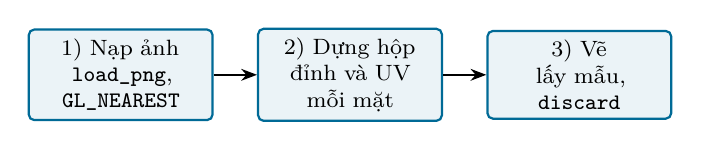
\begin{tikzpicture}[node distance=5.5mm]
\node[pbox] (a) {1) Nạp ảnh \\ \code{load\_png}, \code{GL\_NEAREST}};
\node[pbox,right=of a] (b) {2) Dựng hộp \\ đỉnh và UV mỗi mặt};
\node[pbox,right=of b] (c) {3) Vẽ \\ lấy mẫu, \code{discard}};
\draw[parr] (a)--(b); \draw[parr] (b)--(c);
\end{tikzpicture}
\caption{Ba bước vẽ skin.}
\label{fig:skinflow}
\end{figure}

\textbf{1) Dựng hộp.} Hộp có tâm $\mathbf{c}$, kích thước $(w,h,d)$ và độ phồng $\delta$. Mỗi góc của mặt là
$\mathbf{p}=\mathbf{c}+\big(s_x(\tfrac w2+\delta),\,s_y(\tfrac h2+\delta),\,s_z(\tfrac d2+\delta)\big)$, $s_x,s_y,s_z\in\{\pm1\}$.
Hộp được dựng hai lần: lớp nền ($\delta=0$) và lớp áo ($\delta=0{,}25$ cho thân, tay, chân; $0{,}5$ cho mũ). Lớp áo to hơn một chút nên không bị dính vào lớp nền.

\begin{codebox}
\begin{lstlisting}[language=Python,caption={\code{render/avatar\_renderer.py}, \code{\_box}: góc $\mathbf{p}$ của mặt},label={lst:boxcorner}]
(cx, cy, cz), (w, h, d) = centre, size
hx, hy, hz = w / 2 + inflate, h / 2 + inflate, d / 2 + inflate
...
for (sx, sy, sz), (u, v) in zip(_FACES[face], uvs):
    vertices.append((cx + sx * hx, cy + sy * hy, cz + sz * hz, ...))
\end{lstlisting}
\end{codebox}

\textbf{2) Chọn ô trên ảnh.} Hộp có gốc $(o_x,o_y)$ trên skin. Hình~\ref{fig:skincross} cho thấy sáu mặt nằm ở đâu. Ví dụ đầu có gốc $(0,0)$ và $w=h=d=8$, nên mặt trước (khuôn mặt) nằm ở ô $(8,8,8,8)$. Bốn góc của ô $(r_x,r_y,r_w,r_h)$ nhận UV
\begin{equation}
(u,v)=\Big(\tfrac{r_x+k\,r_w}{64},\,\tfrac{r_y+l\,r_h}{64}\Big),\quad (k,l)\in\{(0,0),(1,0),(1,1),(0,1)\}.
\label{eq:skin-uv}
\end{equation}
Thứ tự bốn góc phải khớp với thứ tự bốn đỉnh của mặt, nếu lệch thì ảnh bị lật hoặc xoay.

\begin{codebox}
\begin{lstlisting}[language=Python,caption={\code{render/avatar\_renderer.py}: ô skin của mặt và UV},label={lst:skinuv}]
def _uv_region(face, ox, oy, w, h, d):
    return ((ox + d, oy + d, w, h), (ox + 2 * d + w, oy + d, w, h),
            (ox, oy + d, d, h), (ox + d + w, oy + d, d, h),
            (ox + d, oy, w, d), (ox + d + w, oy, w, d))[face]

rx, ry, rw, rh = _uv_region(face, ox, oy, w, h, d)
uvs = ((rx, ry), (rx + rw, ry), (rx + rw, ry + rh), (rx, ry + rh))
...  u / SKIN_SIZE, v / SKIN_SIZE
\end{lstlisting}
\end{codebox}

\begin{figure}[H]
\centering
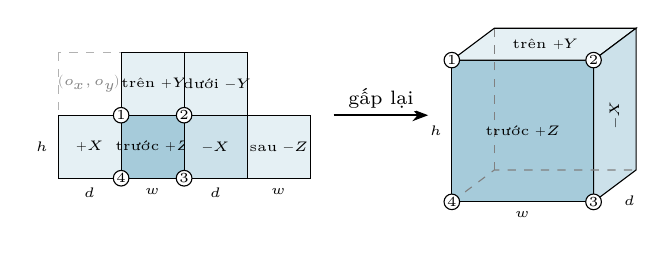
\begin{tikzpicture}[font=\tiny]
% hình chữ thập trên ảnh skin (gốc (o_x,o_y) ở góc trên trái)
\begin{scope}[x=0.4cm,y=-0.4cm]
\draw[dashed,gray!60] (0,0) rectangle (2,2);
\node[gray] at (1,1) {$(o_x,o_y)$};
\draw[fill=linkblue!10] (2,0) rectangle (4,2) node[midway]{trên $+Y$};
\draw[fill=linkblue!10] (4,0) rectangle (6,2) node[midway]{dưới $-Y$};
\draw[fill=linkblue!10] (0,2) rectangle (2,4) node[midway]{$+X$};
\draw[fill=linkblue!35] (2,2) rectangle (4,4) node[midway]{trước $+Z$};
\draw[fill=linkblue!20] (4,2) rectangle (6,4) node[midway]{$-X$};
\draw[fill=linkblue!10] (6,2) rectangle (8,4) node[midway]{sau $-Z$};
\foreach \p/\n in {{2,2}/1,{4,2}/2,{4,4}/3,{2,4}/4}
  \node[circle,fill=white,draw,inner sep=0.3pt] at (\p) {\n};
\node[below] at (1,4) {$d$}; \node[below] at (3,4) {$w$};
\node[below] at (5,4) {$d$}; \node[below] at (7,4) {$w$};
\node[left] at (0,3) {$h$};
\end{scope}
\draw[parr] (3.5,-0.8) -- node[plab,above=1pt]{gấp lại} (4.7,-0.8);
% hộp 3D tương ứng (phép chiếu xiên)
\begin{scope}[shift={(5.0,-1.9)},x=0.9cm,y=0.9cm]
\draw[fill=linkblue!35] (0,0) rectangle (2,2);
\draw[fill=linkblue!10] (0,2) -- (2,2) -- (2.6,2.45) -- (0.6,2.45) -- cycle;
\draw[fill=linkblue!20] (2,0) -- (2.6,0.45) -- (2.6,2.45) -- (2,2) -- cycle;
\draw[dashed,gray] (0,0) -- (0.6,0.45) -- (2.6,0.45); \draw[dashed,gray] (0.6,0.45) -- (0.6,2.45);
\node at (1,1) {trước $+Z$};
\node at (1.3,2.22) {trên $+Y$};
\node[rotate=90] at (2.3,1.22) {$-X$};
\foreach \p/\n in {{0,2}/1,{2,2}/2,{2,0}/3,{0,0}/4}
  \node[circle,fill=white,draw,inner sep=0.3pt] at (\p) {\n};
\node[below] at (1,0) {$w$}; \node[left] at (0,1) {$h$};
\node[below right] at (2.3,0.22) {$d$};
\end{scope}
\end{tikzpicture}
\caption{Hộp 3D và hình chữ thập của nó. Mặt $+Z$ ($w\times h$) có ô $(o_x{+}d,\,o_y{+}d,\,w,\,h)$, mặt $+Y$ có ô $(o_x{+}d,\,o_y,\,w,\,d)$. Bốn góc 1, 2, 3, 4 của mỗi mặt nhận $(k,l)=(0,0),(1,0),(1,1),(0,1)$ trong \eqref{eq:skin-uv}.}
\label{fig:skincross}
\end{figure}

\textbf{3) Vẽ.} Skin được nạp bằng hàm \code{load\_png} tự viết và lọc \code{GL\_NEAREST}, nên pixel giữ nguyên độ sắc nét ($\lfloor 64u\rfloor,\lfloor 64v\rfloor$). Fragment shader bỏ pixel có $\alpha<0{,}5$, nhờ đó chỗ trong suốt của lớp áo để lộ lớp nền. Màu cuối bằng màu texel nhân $0{,}62+0{,}38\max(\mathbf{n}\!\cdot\!\mathbf{l},0)$. Mỗi hộp được vẽ với ma trận model riêng, nên tay và chân xoay độc lập quanh khớp.

\begin{figure}[H]
\centering

\includegraphics[width=0.45\columnwidth]{figures/skinzom.png}
\caption{Skin $64\times64$ của nhân vật. Mỗi hộp (đầu, thân, tay, chân) có một hình chữ thập cho lớp nền và một hình cho lớp áo (mũ, áo, tay áo).}
\label{fig:skin}
\end{figure}

%====================================================================
\section{T4: Ánh sáng và bóng đổ}
\label{chap:t4}
%====================================================================
Màu cuối của một gaussian được tạo qua bốn phần.
\begin{itemize}\itemsep0pt
\item \textbf{Phần 1, màu phụ thuộc hướng nhìn.} Đọc màu gốc từ các hệ số SH.
\item \textbf{Phần 2, chiếu sáng Phong.} Cộng ánh sáng môi trường, khuếch tán và phản chiếu.
\item \textbf{Phần 3, mặt trời.} Di chuyển mặt trời và màu trời theo giờ.
\item \textbf{Phần 4, bóng đổ.} Kiểm tra từng gaussian với shadow map.
\end{itemize}

\subsection{Phần 1: Màu phụ thuộc hướng nhìn}
\label{sec:sh}
Màu của một gaussian thay đổi theo hướng nhìn $\mathbf{d}$. 3DGS lưu điều này bằng các hệ số điều hòa cầu (SH) \cite{kerbl2023gaussian}:
\begin{equation}
\mathbf{c}(\mathbf{d})=\operatorname{clip}\!\Big(\mathbf{c}_0+\sum_{k=1}^{K}Y_k(\mathbf{d})\,\mathbf{h}_k,\,0,\,1\Big).
\label{eq:sh}
\end{equation}
Ở đây $\mathbf{c}_0$ là màu cơ bản, $\mathbf{h}_k$ là các hệ số trong file và $Y_k$ là các hàm cơ sở. Các hệ số nằm trong không gian file. Vì vậy shader quay hướng nhìn về không gian đó: $\mathbf{d}=\operatorname{norm}\!\big(\mathbf{A}^{\top}(\mathbf{p}_w-\mathbf{e})\big)$. Nó không phải quay các hệ số trong mỗi khung hình. Hình~\ref{fig:sh} minh họa ý tưởng cho bậc 0 đến 2. Mỗi hàm cơ sở là một mẫu hình trên mặt cầu. Tổng có trọng số cho một màu ứng với mỗi hướng nhìn.

\begin{codebox}
\begin{lstlisting}[language=GLSL,caption={\code{render/shaders/splat\_prep.vert}: màu SH theo hướng nhìn},label={lst:sh}]
vec3 c = -0.4886025119029199 * y * shCoeff(splat, 0)
       +  0.4886025119029199 * z * shCoeff(splat, 1)
       -  0.4886025119029199 * x * shCoeff(splat, 2);
...
vec3 color = vec3(rg, ba.x);
if (uShDegree > 0)
    color += shColor(splat, normalize(transpose(linear)
                                      * (center - uCamPos)));
color = clamp(color, 0.0, 1.0);
\end{lstlisting}
\end{codebox}

\begin{figure}[H]
\centering
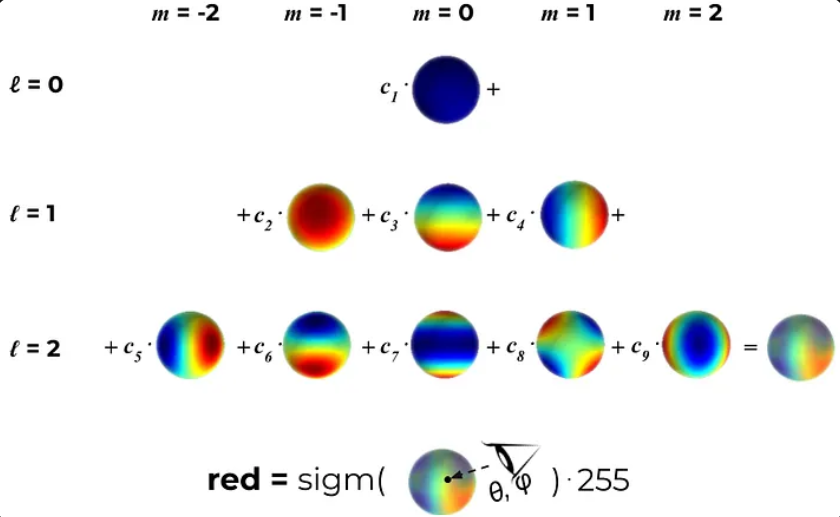
\includegraphics[width=0.8\columnwidth]{figures/1 (1).png}
\caption{Điều hòa cầu đến bậc 2. Chín hàm cơ sở được nhân với các hệ số $c_1..c_9$ rồi cộng lại. Màu được đọc tại hướng nhìn $(\theta,\varphi)$.}
\label{fig:sh}
\end{figure}

\subsection{Phần 2: Chiếu sáng Phong}
Ánh sáng được tính một lần cho mỗi gaussian. Pháp tuyến $\mathbf{n}$ là trục ngắn nhất của ellipsoid, lật về phía camera. Màu cuối dùng mô hình Phong \cite{phong1975}. Mô hình có ba phần (Hình~\ref{fig:phong}). Gọi $\mathbf{c}$ là màu của gaussian.

\textbf{Ambient.} Ánh sáng môi trường $\mathbf{L}_a$ chiếu đều lên mọi gaussian:
\begin{equation}
\mathbf{I}_a=\mathbf{c}\,\mathbf{L}_a.
\label{eq:phong-a}
\end{equation}

\textbf{Diffuse.} Mặt hướng về đèn thì sáng hơn. Với đèn $j$, $\mathbf{L}_j$ là màu và $\mathbf{l}_j$ là hướng về đèn:
\begin{equation}
\begin{aligned}
\mathbf{I}_d&=\mathbf{c}\sum_j \mathbf{L}_j\,w(\mathbf{n},\mathbf{l}_j)\,S_j,\\
w(\mathbf{n},\mathbf{l})&=\operatorname{clip}\!\Big(\frac{\mathbf{n}\!\cdot\!\mathbf{l}+0{,}35}{1{,}35},0,1\Big).
\end{aligned}
\label{eq:phong-d}
\end{equation}
$w$ là $\mathbf{n}\!\cdot\!\mathbf{l}$ đã làm mềm, vì pháp tuyến ước lượng khá nhiễu.

\textbf{Specular.} Điểm sáng bóng hiện ra khi tia phản xạ $\mathbf{r}_j$ gần với hướng $\mathbf{v}$ về camera:
\begin{equation}
\mathbf{I}_s=k_s\sum_{j}\mathbf{L}_j\,(\mathbf{r}_j\!\cdot\!\mathbf{v})_{+}^{m}\,S_j.
\label{eq:phong-s}
\end{equation}
Ở đây $k_s$ là cường độ specular và $m$ là độ bóng. Phần này không dùng màu $\mathbf{c}$. Nó bằng 0 khi $\mathbf{n}\!\cdot\!\mathbf{l}_j\le0$.

\textbf{Tổng.} Màu cuối là tổng của ba phần:
\begin{equation}
\mathbf{c}_{out}=\mathbf{I}_a+\mathbf{I}_d+\mathbf{I}_s.
\label{eq:phong-wrap}
\end{equation}
$S_j$ là hệ số bóng đổ của mặt trời, hoặc độ suy giảm theo khoảng cách của đèn điểm. Cảnh có một mặt trời và tối đa 8 đèn điểm. Đèn điểm không đổ bóng.

\begin{codebox}
\begin{lstlisting}[language=GLSL,caption={\code{render/shaders/splat\_prep.vert}, \code{shade}: Phong},label={lst:phong}]
vec3 diffuse = uAmbient;
vec3 spec = vec3(0.0);
float ndl = dot(n, uSunDir);
float shadow = shadowFactor(worldPos, n);
diffuse += uSunColor * shadow
         * clamp((ndl + 0.35) / 1.35, 0.0, 1.0);
if (ndl > 0.0)
    spec += uSunColor * shadow * pow(max(dot(
        reflect(-uSunDir, n), v), 0.0), uShininess);
...
return albedo * diffuse + spec * uSpecular;
\end{lstlisting}
\end{codebox}

\begin{figure}[H]
\centering
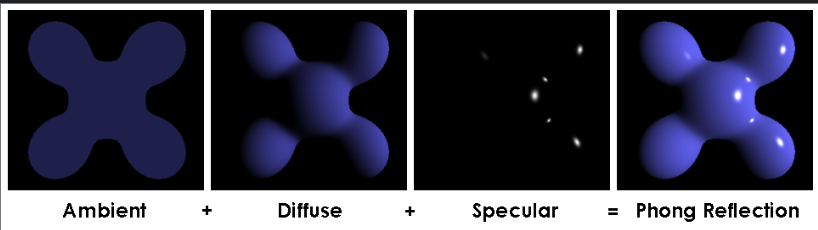
\includegraphics[width=\columnwidth]{figures/1 (2).png}
\caption{Mô hình Phong \cite{phong1975}: phần ambient, diffuse và specular, và tổng của chúng.}
\label{fig:phong}
\end{figure}

\subsection{Phần 3: Mặt trời}
Hướng mặt trời tính từ giờ $h$ trong ngày. Mặt trời mọc lúc 6 giờ, cao nhất lúc 12 giờ và lặn lúc 18 giờ. Màu trời và ánh sáng môi trường đổi dần giữa ngày và đêm. Chúng hơi cam lúc hoàng hôn (Hình~\ref{fig:t4}).

\subsection{Phần 4: Bóng đổ}
Chương trình vẽ tâm các gaussian đặc thành điểm vào một depth map $2048^2$ nhìn từ mặt trời \cite{williams1978}. Mỗi gaussian được chiếu vào map này để so độ sâu. Nếu có vật gần mặt trời hơn, gaussian nằm trong bóng. Chương trình lấy trung bình $3\times3$ mẫu để làm mềm cạnh bóng (PCF \cite{reeves1987}):
\begin{equation}
S=\frac19\sum_{i,j=-1}^{1}\big[\,z_s-b\le D_s(u_s+i\tau,\,v_s+j\tau)\,\big].
\label{eq:pcf}
\end{equation}
Ở đây $(u_s,v_s,z_s)$ là tọa độ của gaussian trong map, $D_s$ là độ sâu đã lưu, $\tau$ là bước texel và $b$ là bias. Bias ngăn gaussian tự đổ bóng lên chính nó.

\begin{codebox}
\begin{lstlisting}[language=GLSL,caption={\code{render/shaders/splat\_prep.vert}, \code{shadowFactor}: PCF $3\times3$},label={lst:pcf}]
vec4 lp = uLightVP * vec4(worldPos + n * uShadowTexel * 2.0, 1.0);
vec3 s = lp.xyz / lp.w * 0.5 + 0.5;
float lit = 0.0;
for (int i = -1; i <= 1; i++)
    for (int j = -1; j <= 1; j++) {
        vec2 uv = s.xy + vec2(i, j) * uShadowInv;
        float d = textureLod(uShadowMap, uv, 0.0).r;
        lit += (s.z - uShadowBias <= d) ? 1.0 : 0.0;
    }
return lit / 9.0;
\end{lstlisting}
\end{codebox}

\begin{codebox}
\begin{lstlisting}[language=Python,caption={\code{core/lighting.py}, \code{Lighting.shadow\_setup}: ma trận nhìn từ mặt trời},label={lst:shadowsetup}]
d = self.sun_direction()
r = self.radius * 1.1
eye = self.center + d * 2.0 * r
view = look_at(eye, self.center, up)
proj = orthographic(r, 0.01 * r, 4.0 * r)
return (proj @ view).astype(np.float32), texel, bias
\end{lstlisting}
\end{codebox}

%====================================================================
\section{T5: Hoạt họa và mô phỏng}
\label{chap:t5}
%====================================================================
Mọi chuyển động đều nhân với thời gian khung hình $\Delta t$. Nhờ vậy tốc độ ít phụ thuộc vào máy. Có bốn phần, theo thứ tự trong một khung hình.
\begin{itemize}\itemsep0pt
\item \textbf{Phần 1, chu kỳ ngày--đêm.} Chạy đồng hồ và di chuyển mặt trời.
\item \textbf{Phần 2, va chạm voxel.} Biến các gaussian thành voxel đặc.
\item \textbf{Phần 3, người chơi.} Đi, nhảy và rơi trên các voxel.
\item \textbf{Phần 4, hoạt họa nhân vật.} Tính góc các khớp của nhân vật.
\end{itemize}

\subsection{Phần 1: Chu kỳ ngày--đêm}
Đây là một máy trạng thái có 4 trạng thái: NIGHT $\to$ DAWN $\to$ DAY $\to$ DUSK. Đồng hồ tự chạy. Đèn đặt ``bật vào ban đêm'' sẽ bật lúc hoàng hôn và tắt lúc bình minh. Các trạng thái bắt đầu lúc 5 giờ (DAWN), 7 giờ (DAY), 17 giờ (DUSK) và 19 giờ (NIGHT). Một ngày dài $T_{day}=36$ giây, nên mỗi khung hình giờ tăng $\Delta h = 24\,\Delta t/T_{day}$. Vị trí mặt trời phụ thuộc vào giờ:
\begin{equation}
\begin{gathered}
\theta=\frac{h-6}{12}\pi,\qquad
\epsilon=65^{\circ}\sin\theta,\
\mathbf{s}=\big(\cos\epsilon\cos\phi,\;\sin\epsilon,\;\cos\epsilon\sin\phi\big),
\end{gathered}
\label{eq:sun}
\end{equation}
trong đó $\phi=\phi_0+\theta-\pi/2$ và $\phi_0$ là góc phương vị của mặt trời. Mặt trời mọc lúc 6 giờ, cao nhất lúc 12 giờ và lặn lúc 18 giờ. Hệ số ánh sáng ngày là $D=\operatorname{smoothstep}(-0{,}08,\,0{,}3,\,s_y)$. Màu môi trường và màu bầu trời được trộn giữa giá trị ban đêm và ban ngày theo $D$, bầu trời có thêm sắc cam gần đường chân trời.

\begin{codebox}
\begin{lstlisting}[language=Python,caption={\code{core/lighting.py}: giờ, hướng mặt trời và hệ số ánh sáng ngày},label={lst:sun}]
hours_per_second = 24.0 / max(self.day_length, 1.0)
self.hour = (self.hour + dt * hours_per_second) % 24.0

angle = (self.hour - 6.0) / 12.0 * math.pi
elevation = math.sin(angle) * math.radians(MAX_SUN_ELEVATION)
azimuth = (math.radians(self.sun_azimuth)
           + (angle - math.pi / 2))
return np.array([math.cos(elevation) * math.cos(azimuth),
                 math.sin(elevation),
                 math.cos(elevation) * math.sin(azimuth)])

return _smooth(-0.08, 0.3, self.sun_direction()[1])
\end{lstlisting}
\end{codebox}

\subsection{Phần 2: Va chạm với voxel}
Gaussian không có bề mặt rõ ràng, nên khó tính va chạm trực tiếp. Chương trình chia không gian thành các voxel cạnh $v$. Voxel có đủ gaussian là voxel đặc. Mỗi voxel đặc được lưu thành một số nguyên 64 bit:
\begin{equation}
\mathbf{c} = \left\lfloor \frac{\mathbf{p}-\mathbf{o}}{v} \right\rfloor,
\qquad
\text{key} = (c_x \ll 42)\,|\,(c_z \ll 21)\,|\,c_y.
\label{eq:voxel}
\end{equation}
Các khóa được sắp xếp. Vì $c_y$ nằm ở các bit thấp, các ô cùng một cột đứng liền nhau. Tìm mặt đất dưới chân chỉ cần một lệnh \code{np.searchsorted}.

\begin{codebox}
\begin{lstlisting}[language=Python,caption={\code{core/physics.py}, \code{CollisionWorld}: khóa voxel và tìm mặt đất},label={lst:voxel}]
cells = np.floor((positions - self.origin) / self.voxel).astype(np.int64)
keys = (cells[:, 0] << (2 * _BITS)) | (cells[:, 2] << _BITS) | cells[:, 1]
self.keys = np.unique(keys)

idx = np.searchsorted(self.keys, query, side='right') - 1
\end{lstlisting}
\end{codebox}

\begin{figure}[H]
\centering
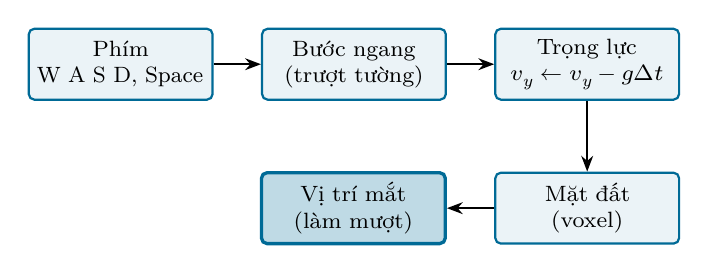
\begin{tikzpicture}[node distance=9mm and 6mm]
  \node[pbox] (key) {Phím\\W A S D, Space};
  \node[pbox,right=of key] (move) {Bước ngang\\(trượt tường)};
  \node[pbox,right=of move] (grav) {Trọng lực\\$v_y\leftarrow v_y-g\Delta t$};
  \node[pbox,below=of grav] (gr) {Mặt đất\\(voxel)};
  \node[pmine,left=of gr] (eye) {Vị trí mắt\\(làm mượt)};
  \draw[parr] (key) -- (move);
  \draw[parr] (move) -- (grav);
  \draw[parr] (grav) -- (gr);
  \draw[parr] (gr) -- (eye);
\end{tikzpicture}
\caption{Một khung hình của chế độ đi bộ.}
\label{fig:t5}
\end{figure}

\subsection{Phần 3: Người chơi}
Hình~\ref{fig:t5} tóm tắt một khung hình. Người chơi là một hình trụ. Khi gặp tường, người chơi trượt dọc theo tường. Người chơi leo được bậc thấp và nhảy được.

\textbf{Trọng lực.} Khi không đứng trên đất, chương trình tích phân theo Euler:
\begin{equation}
v_y \leftarrow v_y - g\,\Delta t,
\qquad
y \leftarrow y + v_y\,\Delta t.
\label{eq:euler}
\end{equation}
\textbf{Tỉ lệ và cú nhảy.} Mọi kích thước và tốc độ tỉ lệ theo chiều cao người chơi $H$. Lý do là cảnh 3DGS không có đơn vị cố định. Các hằng số là: cạnh voxel $v=H/8$, bán kính người chơi $0{,}14H$, chiều cao bậc $0{,}35H$, trọng lực $g=12H$, tốc độ đi $2{,}5H$ mỗi giây (chạy nhanh $\times1{,}7$, đi chậm $\times0{,}4$). Cú nhảy đạt độ cao $0{,}75H$, nên vận tốc lúc bật lên là
\begin{equation}
v_0=\sqrt{2\,g\,(0{,}75H)}.
\label{eq:jump}
\end{equation}
\textbf{Làm mượt mắt.} Độ cao mắt được làm mượt khi người chơi đứng trên đất, để bề mặt gaussian gồ ghề không làm rung camera.

\begin{codebox}
\begin{lstlisting}[language=Python,caption={\code{core/physics.py}, \code{Physics.walk}: nhảy và trọng lực},label={lst:jump}]
if player.on_ground and jump:
    player.vel_y = math.sqrt(2.0 * self.gravity * self.jump_ratio * h)
    player.on_ground = False
if not player.on_ground:
    player.vel_y -= self.gravity * dt
    new_y = y + player.vel_y * dt
\end{lstlisting}
\end{codebox}

\subsection{Phần 4: Hoạt họa nhân vật}
Chương trình chỉ tính góc các khớp (đơn vị độ); renderer dựng ma trận. Gọi $d$ là quãng đường đi được trong khung hình này, tính theo chiều cao người. Pha của bước đi tăng theo quãng đường chứ không theo thời gian, nên chân không bị trượt trên đất:
\begin{equation}
\psi\leftarrow\psi+1{,}75\cdot2\,d,\qquad
\theta_{chân}=\pm A\,a\,\sin\psi,\quad
\theta_{tay}=\mp A\,a\,\sin\psi,
\label{eq:gait}
\end{equation}
với $A=60^{\circ}$. Chân và tay đối diện chuyển động cùng nhau.

\textbf{Trộn trạng thái.} Biên độ $a\in[0,1]$ bám theo tốc độ bằng bộ lọc $x\leftarrow x+(x^{*}-x)\min(1,k\,\Delta t)$ \eqref{eq:fly}, với $k=8$. Cùng bộ lọc này, với $k=7$, trộn các trạng thái khác: ngồi (chân $-90^{\circ}$, thân hạ xuống), cúi (thân nghiêng $28^{\circ}$) và các cử chỉ vẫy tay, zombie, cổ vũ. Hai tư thế được trộn tuyến tính, $\theta=(1-w)\theta_a+w\,\theta_b$, nên cử chỉ hiện ra và mất đi mượt. Khi đứng yên, một số hạng $\sin$ nhỏ làm tay lắc nhẹ để giả lập nhịp thở.

\begin{codebox}
\begin{lstlisting}[language=Python,caption={\code{core/avatar\_pose.py}: nhịp đi và bộ lọc làm mượt},label={lst:gait}]
def _approach(value, target, rate, dt):
    return value + (target - value) * min(1.0, dt * rate)

walked = distance / max(height, 1e-9)
self.amount = _approach(self.amount, target, BLEND, dt)
self.phase += walked * STRIDE * GAIT_SCALE
swing = math.sin(self.phase) * SWING_ANGLE * walk
leg_l, leg_r = swing, -swing
arm_l = [-swing + idle, 0.0]
arm_r = [swing - idle, 0.0]
\end{lstlisting}
\end{codebox}

\textbf{Ma trận khớp.} Mỗi chi là một phép quay quanh khớp của nó: $\mathbf{M}=\mathbf{T}(\mathbf{j})\,\mathbf{R}(\theta)\,\mathbf{T}(-\mathbf{j})$, nhân sau ma trận của khối cha, ví dụ tay nhân sau thân.

%====================================================================
\section{T6: Tương tác và giao diện}
\label{chap:t6}
%====================================================================
Tương tác có bốn phần, từ đầu vào đến màn hình.
\begin{itemize}\itemsep0pt
\item \textbf{Phần 1, xử lý sự kiện.} Quyết định ai nhận mỗi sự kiện chuột hoặc phím.
\item \textbf{Phần 2, chọn bằng cọ.} Chọn gaussian bằng cách tô lên màn hình.
\item \textbf{Phần 3, xóa mềm và hoàn tác.} Xóa vùng chọn và khôi phục.
\item \textbf{Phần 4, giao diện.} Bảng điều khiển, HUD và phím tắt.
\end{itemize}

\subsection{Phần 1: Xử lý sự kiện}
Sự kiện chuột và bàn phím đến ImGui trước. Nếu ImGui không dùng, chúng đến camera, cọ chọn và các phím tắt.

\subsection{Phần 2: Chọn bằng cọ}
Nhấn \code{B} để bật cọ. Tô lên màn hình để chọn gaussian. Chúng chuyển sang màu vàng. Tâm mỗi gaussian được chiếu thành pixel $\mathbf{p}$ (Mục~\ref{sec:cam}). 

\textbf{Kiểm tra capsule.} Một nét vẽ từ $\mathbf{a}$ đến $\mathbf{b}$ là một capsule bán kính $r$. Gaussian được chọn nếu
\begin{equation}
\lVert\mathbf{p}-\mathbf{a}-\tau(\mathbf{b}-\mathbf{a})\rVert\le r,\quad \tau=\operatorname{clip}\tfrac{(\mathbf{p}-\mathbf{a})\cdot(\mathbf{b}-\mathbf{a})}{\lVert\mathbf{b}-\mathbf{a}\rVert^2}\in[0,1].
\label{eq:capsule}
\end{equation}
Tức là khoảng cách từ $\mathbf{p}$ đến đoạn $\mathbf{ab}$ không quá $r$.

\begin{codebox}
\begin{lstlisting}[language=Python,caption={\code{editor/brush.py}, \code{BrushTool.\_segment\_dist2}: kiểm tra capsule},label={lst:capsule}]
def _segment_dist2(p, a, b):
    ab = b - a
    length2 = float(ab @ ab)
    t = (np.clip((p - a) @ ab / length2, 0, 1) if length2 > 0
         else np.zeros(p.shape[:-1]))
    nearest = a + t[..., None] * ab
    diff = p - nearest
    return (diff * diff).sum(axis=-1)
\end{lstlisting}
\end{codebox} 

\textbf{Tính chất.} Cọ chỉ xét tâm gaussian và không kiểm tra độ sâu. Vì vậy nó chọn xuyên qua cảnh, giống SuperSplat \cite{supersplat}. Để nhanh, cọ loại cả khối 1024 gaussian khi hộp bao của khối nằm ngoài nét vẽ.

\subsection{Phần 3: Xóa mềm và hoàn tác}
Mỗi gaussian có một byte trạng thái trên GPU với hai bit: \emph{đã chọn} và \emph{đã xóa}. Lệnh \code{Delete} chỉ bật bit ``đã xóa''. Shader bỏ qua các gaussian này. Dữ liệu gốc không đổi. Mỗi lần xóa là một lệnh trong \code{History} (mẫu Command \cite{gamma1994design}, tối đa 20 bước). \code{Ctrl+Z} khôi phục lệnh cuối.

\begin{codebox}
\begin{lstlisting}[language=Python,caption={\code{core/layer.py} và \code{core/history.py}: xóa mềm và hoàn tác},label={lst:history}]
def delete_selected(self):
    indices = np.flatnonzero(self.selection)
    self.deleted[indices] = True
    self.selection[indices] = False
    return indices

def push(self, command):
    self._stack.append(command)
    del self._stack[:-self.max_steps]

def undo(self):
    command = self._stack.pop()
    command.undo()
\end{lstlisting}
\end{codebox}

\subsection{Phần 4: Giao diện}
Bảng ImGui bên trái điều khiển layer, phép biến đổi, vùng chọn, chế độ camera và ánh sáng. HUD hiển thị tâm ngắm, đồng hồ, vị trí và vòng tròn cọ. Bảng~\ref{tab:keys} liệt kê các phím chính.
\begin{table}[H]
\centering
\caption{Các phím điều khiển chính.}
\label{tab:keys}
\footnotesize
\begin{tabular}{@{}p{3.1cm}p{4.6cm}@{}}
\toprule
Phím / chuột & Chức năng \\
\midrule
Kéo chuột trái / giữa & Xoay quanh / pan \\
Kéo chuột phải + \code{WASD} & Nhìn quanh, bay (\code{Ctrl} = nhanh) \\
\code{M}, \code{F5}, \code{C}, \code{V} & Bay/đi bộ; góc nhìn thứ ba; ngồi; vẫy tay \\
\code{F}, \code{G} & Xem toàn cảnh; hiện/ẩn lưới \\
\code{B}, \code{[}, \code{]} & Cọ chọn; cỡ cọ \\
\code{Delete}, \code{Ctrl+Z} & Xóa / hoàn tác \\
\code{Ctrl+O/I/S} & Mở / thêm layer / lưu \\
\bottomrule
\end{tabular}
\end{table}

%====================================================================
\section{Hạn chế và hướng phát triển}
\label{chap:future}
%====================================================================
\subsection{Hạn chế}
\begin{itemize}\itemsep0pt
\item \textbf{Tốc độ phụ thuộc CPU.} Độ sâu được sắp xếp bằng NumPy trong một luồng nền (Mục~\ref{sec:blend}). Khi camera quay nhanh, hình có thể nhấp nháy, và cảnh lớn phải giới hạn số gaussian vẽ (LOD).
\item \textbf{Hình học xấp xỉ.} Gaussian không có bề mặt thật. Cọ chọn, va chạm, pháp tuyến và bóng đều dựa vào tâm gaussian, nên cọ chọn cả vật bị che, va chạm có thể thủng lỗ và ánh sáng còn thô.
\end{itemize}

\subsection{Hướng phát triển}
\begin{itemize}\itemsep0pt
\item \textbf{Hỗ trợ mô phỏng.} Dùng bản đồ voxel và phần vật lý có sẵn để mô phỏng chuyển động trong cảnh quay từ đời thực, ví dụ thử đường đi của người, robot hay xe. Cần va chạm chính xác hơn và thêm các vật thể động.
\item \textbf{Ứng dụng vào game.} Biến cảnh 3DGS thành một màn chơi: thêm nhân vật máy, vật phẩm và nhiệm vụ, giữ chu kỳ ngày đêm và đèn. Cảnh đã làm sạch có thể xuất sang game engine như Unity hoặc Unreal.
\end{itemize}

%====================================================================
\section{Tuyên bố sử dụng AI}
\label{chap:ai}
%====================================================================
Theo quy định của môn học, sinh viên được dùng công cụ AI (ChatGPT, Gemini) để học khái niệm, gỡ lỗi và cải thiện mã nguồn. Trong đồ án này, tôi đã dùng ChatGPT và Gemini cho hai việc:
\begin{itemize}\itemsep0pt
\item \textbf{Học khái niệm.} Giải thích 3D Gaussian Splatting, EWA, điều hòa cầu, bản đồ bóng và các kỹ thuật đồ họa liên quan.
\item \textbf{Gỡ lỗi và cải thiện mã.} Tìm lỗi, gợi ý cách viết gọn và nhanh hơn cho chương trình.
\end{itemize}
Tôi đã đọc, kiểm tra và chạy thử nội dung do AI gợi ý, và chịu trách nhiệm về toàn bộ mã nguồn và báo cáo này.

%====================================================================
\section{Kết luận}
\label{chap:end}
%====================================================================
Splat Editor đọc, hiển thị, chỉnh sửa và lưu được file 3DGS. Chương trình dùng đủ sáu nhóm kỹ thuật của môn học. Bảng~\ref{tab:src} chỉ vị trí của từng phần trong mã nguồn.

\begin{table}[H]
\centering
\caption{Các file mã nguồn chính (trong \code{splat\_editor/}).}
\label{tab:src}
\footnotesize
\begin{tabular}{@{}p{2.2cm}>{\raggedright\arraybackslash}p{5.5cm}@{}}
\toprule
Phần & File \\
\midrule
Đọc/ghi PLY & \mbox{\code{io/ply.py}}, \mbox{\code{io/codec.py}} \\
Hiển thị gaussian & \mbox{\code{render/splat\_renderer.py}}, \mbox{\code{render/sorter.py}}, \mbox{\code{render/shaders/splat\_prep.vert}} \\
T1 & \mbox{\code{core/layer.py}}, \mbox{\code{core/transform.py}}, \mbox{\code{core/avatar\_pose.py}} \\
T2 & \mbox{\code{core/math3d.py}}, \mbox{\code{render/camera.py}} \\
T3 & \mbox{\code{render/avatar\_renderer.py}} \\
T4 & \mbox{\code{core/sh.py}}, \mbox{\code{core/lighting.py}}, \mbox{\code{render/shaders/shadow.vert}} \\
T5 & \mbox{\code{core/physics.py}}, \mbox{\code{core/avatar\_pose.py}} \\
T6 & \mbox{\code{editor/brush.py}}, \mbox{\code{core/history.py}}, \mbox{\code{ui/}} \\
\bottomrule
\end{tabular}
\end{table}

\begin{thebibliography}{99}\footnotesize\itemsep0pt\parskip0pt
\bibitem{schonberger2016colmap} J.~L.~Sch{\"o}nberger, J.-M.~Frahm, Structure-from-motion revisited, in: CVPR, 2016, pp.~4104--4113.
\bibitem{kerbl2023gaussian} B.~Kerbl, G.~Kopanas, T.~Leimk{\"u}hler, G.~Drettakis, 3D Gaussian splatting for real-time radiance field rendering, ACM Trans. Graph. 42(4) (2023) 139.
\bibitem{supersplat} PlayCanvas, SuperSplat: an open-source 3D Gaussian Splat editor, \url{https://github.com/playcanvas/supersplat}.
\bibitem{zwicker2002ewa} M.~Zwicker, H.~Pfister, J.~van Baar, M.~Gross, EWA splatting, IEEE Trans. Vis. Comput. Graph. 8(3) (2002) 223--238.
\bibitem{phong1975} B.~T.~Phong, Illumination for computer generated pictures, Commun. ACM 18(6) (1975) 311--317.
\bibitem{williams1978} L.~Williams, Casting curved shadows on curved surfaces, in: SIGGRAPH, 1978, pp.~270--274.
\bibitem{reeves1987} W.~T.~Reeves, D.~H.~Salesin, R.~L.~Cook, Rendering antialiased shadows with depth maps, in: SIGGRAPH, 1987, pp.~283--291.
\bibitem{gamma1994design} E.~Gamma, R.~Helm, R.~Johnson, J.~Vlissides, Design Patterns: Elements of Reusable Object-Oriented Software, Addison-Wesley, 1994.
\end{thebibliography}

\end{document}
